\chapter{Series and Convolution}
\label{chap:series_conv}
\markboth{Series and Convolution}{Series and Convolution}

\begin{remark}[Positioning of This Chapter]\label{rem:series_chapter_positioning}
This chapter builds the complete theory of \textbf{series} and \textbf{convolution}. A series is the decomposition of a function into countably many elementary units: the Taylor series (the local derivative spectrum), the Laurent series (a complex expansion containing negative powers), the Fourier series (a global frequency decomposition on the harmonic lattice) and the periodic series (a complex series whose components are amplitude, frequency, phase and period, with the period as the primary index). Convolution is a function operator that takes two functions together with a delay and computes the delay product; its frequency-domain forms---\textbf{phase convolution}, \textbf{amplitude convolution}, \textbf{frequency convolution} and \textbf{periodic convolution}---lift the similarity/trend hierarchy of the `Scalars and Vectors' chapter to complex matrices between frequency pairs.

Series are the ultimate destination of similarity and trend at the level of the frequency domain: the Fourier coefficients and the Bohr coefficients are given by integrals (trend), whilst the Taylor coefficients are given by derivatives (direction). All classical integral transforms---the Fourier transform, the Mellin transform, the Laplace transform, the wavelet transform and the Chirp-Z transform---are special cases of the periodic transform under a particular frequency dictionary or kernel.

Finally, this chapter establishes the formal definition of \textbf{periodic convolution}: periodic convolution takes amplitude, frequency, phase and period as its four parameters, preserves the interaction of all frequency pairs and all period pairs, and is the summit of the five-stage ladder of convolution theory (convolution $\to$ phase convolution/amplitude convolution/frequency convolution $\to$ trend convolution $\to$ periodic series $\to$ periodic convolution).

\textbf{Guide to the seven themes of this chapter}: translation---the local translation expansion of the Taylor series and the global translation period of the Fourier series; scaling---amplitude (scaling) and period (fixed length); rotation---phase (rotation) and frequency (ordering); conservation---Parseval's identity (conservation of energy) and Bohr's generalised Parseval identity; symmetry---the positive--negative power symmetry of the Laurent series and the orthogonal symmetry of the Fourier basis; closure---the uniqueness of the coefficients of the periodic series (Bohr's theorem); period---the four-tuple structure of the periodic series and periodic convolution.
\end{remark}

\section{\texorpdfstring{Basic Concepts of Series}{Basic Concepts of Series}}

\begin{definition}[Series and Convergence]\label{def:series_basic}
Let $\{a_k\}_{k=0}^{\infty}$ be a sequence of numbers. The formal sum $\sum_{k=0}^{\infty} a_k$ is called a \textbf{series}, with partial sums $S_n = \sum_{k=0}^{n} a_k$. If $\lim_{n\to\infty} S_n = S$ exists, the series \textbf{converges} to $S$; otherwise it \textbf{diverges}. If $\sum_k |a_k|$ converges, the original series is said to \textbf{converge absolutely}; one that converges but does not converge absolutely is said to \textbf{converge conditionally}.
\end{definition}

\begin{definition}[Series of Functions and Uniform Convergence]\label{def:series_of_functions}
Let $\{u_k(t)\}$ be a sequence of functions on $I \subseteq \mathbb{R}$. The series of functions $\sum_k u_k(t)$ is said to \textbf{converge pointwise} to $f$ on $I$ if $f(t) = \sum_k u_k(t)$ for every $t \in I$; it is said to \textbf{converge uniformly} to $f$ if
\[
\lim_{n \to \infty} \sup_{t \in I} \Big| f(t) - \sum_{k=0}^{n} u_k(t) \Big| = 0.
\]
\end{definition}

\begin{proposition}[Ratio Test and Root Test]\label{prop:ratio_root_tests}
Let $a_k \neq 0$. If one of the following limits exists:
\[
\lim_{k\to\infty} \left| \frac{a_{k+1}}{a_k} \right| = \rho,
\qquad\text{or}\qquad
\lim_{k\to\infty} \sqrt[k]{|a_k|} = \rho,
\]
then
\[
\begin{aligned}
\rho < 1 &\implies \sum_k a_k \ \text{converges absolutely}, \\
\rho > 1 &\implies \sum_k a_k \ \text{diverges}, \\
\rho = 1 &\implies \text{the test is inconclusive}.
\end{aligned}
\]
\end{proposition}

\begin{proof}
\textbf{Ratio test}: let $\rho < 1$. Choose $r$ with $\rho < r < 1$. There exists $N$ such that $|a_{k+1}/a_k| < r$ whenever $k \ge N$. By induction $|a_k| \le |a_N| r^{k-N}$. By the convergence of the geometric series, $\sum_k |a_k|$ converges. If $\rho > 1$, take $1 < r < \rho$; there exists $N$ such that $|a_{k+1}/a_k| > r$ whenever $k \ge N$, hence $|a_k| \to \infty$ and the series diverges. Counterexamples showing failure when $\rho = 1$: the ratio limits of $\sum 1/k$ (divergent) and $\sum 1/k^2$ (convergent) are both $1$.

\textbf{Root test}: similar, using the cases $\sqrt[k]{|a_k|} < r$ or $> r$.
\end{proof}

\begin{theorem}[Weierstrass M-Test]\label{thm:weierstrass_mtest}
Let $\sum_k M_k$ be a convergent series of positive terms, and suppose $|u_k(t)| \le M_k$ for all $t \in I$ and all $k$. Then $\sum_k u_k(t)$ converges uniformly and absolutely on $I$.
\end{theorem}

\begin{proof}
Since $\sum M_k$ converges, for any $\varepsilon > 0$ there exists $N$ such that $\sum_{k>n} M_k < \varepsilon$ ($n \ge N$). For any $t \in I$ and $m > n \ge N$,
\[
\Big| \sum_{k=n+1}^{m} u_k(t) \Big| \le \sum_{k=n+1}^{m} |u_k(t)| \le \sum_{k=n+1}^{m} M_k < \varepsilon.
\]
Hence the sequence of partial sums is uniformly Cauchy on $I$ and therefore converges uniformly; absolute convergence follows from $\sum_k |u_k(t)| \le \sum_k M_k < \infty$.
\end{proof}

\begin{theorem}[Term-by-Term Integration under Uniform Convergence]\label{thm:uniform_termwise_integration}
Let $\sum_k u_k$ converge uniformly to $f$ on $[a,b]$, and suppose each $u_k$ is integrable on $[a,b]$. Then
\[
\int_a^b f(t)\,dt = \sum_{k=0}^{\infty} \int_a^b u_k(t)\,dt.
\]
\end{theorem}

\begin{proof}
Write $S_n = \sum_{k=0}^{n} u_k$. By uniform convergence,
\[
\Big| \int_a^b f - \int_a^b S_n \Big| \le \int_a^b |f - S_n| \le (b-a)\, \sup_{t \in [a,b]} |f(t) - S_n(t)| \to 0.
\]
Also $\int_a^b S_n = \sum_{k=0}^{n} \int_a^b u_k$ (the integral of a finite sum equals the finite sum of the integrals); taking the limit gives the result.
\end{proof}

\begin{theorem}[Term-by-Term Differentiation under Uniform Convergence]\label{thm:uniform_termwise_differentiation}
Suppose each $u_k$ is continuously differentiable on $I$, $\sum_k u_k$ converges pointwise to $f$ on $I$, and $\sum_k u_k'$ converges uniformly on $I$. Then $f$ is differentiable and
\[
f'(t) = \sum_{k=0}^{\infty} u_k'(t).
\]
\end{theorem}

\begin{proof}
Let $\sum_k u_k' = g$ (uniformly convergent). For any $a, t \in I$, by Theorem \ref{thm:uniform_termwise_integration},
\[
\int_a^t g(s)\,ds = \sum_{k=0}^{\infty} \int_a^t u_k'(s)\,ds = \sum_{k=0}^{\infty} \big( u_k(t) - u_k(a) \big) = f(t) - f(a).
\]
By the fundamental theorem of calculus, $f'(t) = g(t) = \sum_k u_k'(t)$.
\end{proof}

\begin{theorem}[Cauchy--Hadamard Radius of Convergence Formula]\label{thm:cauchy_hadamard}
The radius of convergence of the power series $\sum_k a_k (z - z_0)^k$ is
\[
R = \frac{1}{\limsup_{k\to\infty} \sqrt[k]{|a_k|}},
\]
(with the conventions $1/0 = \infty$, $1/\infty = 0$): it converges absolutely when $|z - z_0| < R$ and diverges when $|z - z_0| > R$.
\end{theorem}

\begin{proof}
Let $L = \limsup_k \sqrt[k]{|a_k|}$. By the root test,
\[
\limsup_{k} \sqrt[k]{|a_k|\,|z-z_0|^k} = |z-z_0| \cdot L.
\]
When $|z-z_0| L < 1$, that is $|z-z_0| < 1/L = R$, the root is less than $1$ and the series converges absolutely. When $|z-z_0| L > 1$, the root is greater than $1$, the general term does not tend to zero, and the series diverges.
\end{proof}

\begin{property}[Basic Properties of Convergent Series]\label{prop:series_properties}
\begin{enumerate}[label=(\roman*)]
    \item \textbf{Linearity}: if $\sum_k a_k = A$ and $\sum_k b_k = B$, then $\sum_k (a_k + b_k) = A + B$;
    \item \textbf{The general term tends to zero}: if $\sum_k a_k$ converges, then $a_k \to 0$;
    \item \textbf{Absolute convergence implies convergence}: $\sum_k |a_k|$ converges $\implies$ $\sum_k a_k$ converges.
\end{enumerate}
\end{property}

\begin{proof}
(i) By the linearity of the limit of the partial sums. (ii) $a_n = S_n - S_{n-1} \to S - S = 0$. (iii) The sequence of partial sums $\{\sum_{k=0}^{n} a_k\}$ is Cauchy: for $m > n$, $|\sum_{k=n+1}^m a_k| \le \sum_{k=n+1}^m |a_k|$, and the convergence of $\sum |a_k|$ guarantees that the right-hand side can be made arbitrarily small.
\end{proof}

\begin{example}[The Geometric Series: Prototype of a Series]\label{ex:geometric_series}
\[
\sum_{k=0}^{\infty} r^k = \frac{1}{1-r}, \qquad |r| < 1.
\]
The geometric series is the basic building block of power-series expansions: both the positive-power and the negative-power parts of the Taylor and Laurent expansions are derived by way of the geometric series.
\end{example}

\begin{proposition}[Cauchy convergence criterion]\label{prop:cauchy_criterion_series}
A series of real numbers $\sum_{k=0}^{\infty} a_k$ converges if and only if: for every $\varepsilon > 0$ there exists $N \in \mathbb{N}$ such that for all $m > n \ge N$,
\[
\Big| \sum_{k=n+1}^{m} a_k \Big| < \varepsilon.
\]
\end{proposition}

\begin{proof}
($\Rightarrow$) Let $\sum_k a_k = S$, so that the partial sums $S_n \to S$. For $\varepsilon > 0$ choose $N$ such that $|S_n - S| < \varepsilon/2$ whenever $n \ge N$. Then for $m > n \ge N$,
\[
\Big| \sum_{k=n+1}^{m} a_k \Big| = |S_m - S_n| \le |S_m - S| + |S - S_n| < \varepsilon.
\]
($\Leftarrow$) The condition shows that the sequence of partial sums $\{S_n\}$ is Cauchy. By completeness of the real numbers (Theorem \ref{thm:real_completeness} of the `Number Systems' chapter), $\{S_n\}$ converges, that is, $\sum_k a_k$ converges.
\end{proof}

\begin{proposition}[Comparison test]\label{prop:comparison_test}
Let $\sum_k b_k$ be a convergent series of positive terms. If there exists $N$ such that $|a_k| \le b_k$ for $k \ge N$, then $\sum_k a_k$ converges absolutely. Conversely, if $\sum_k b_k$ diverges and $0 \le b_k \le a_k$ for $k \ge N$, then $\sum_k a_k$ diverges.
\end{proposition}

\begin{proof}
Let $\sum_k b_k$ converge. For $m > n \ge N$,
\[
\sum_{k=n+1}^{m} |a_k| \le \sum_{k=n+1}^{m} b_k.
\]
By the Cauchy criterion for $\sum_k b_k$ (Proposition \ref{prop:cauchy_criterion_series}) the right-hand side can be made arbitrarily small, so $\sum_k |a_k|$ converges. The second part follows by reversing the comparison inequality.
\end{proof}

\begin{proposition}[Integral test]\label{prop:integral_test}
Let $f: [1, \infty) \to [0, \infty)$ be monotonically decreasing and continuous. Then the series $\sum_{k=1}^{\infty} f(k)$ and the improper integral $\int_1^{\infty} f(x)\,dx$ converge or diverge together.
\end{proposition}

\begin{proof}
For $k \le x \le k+1$, monotonic decrease of $f$ gives $f(k+1) \le f(x) \le f(k)$. Integrating,
\[
f(k+1) \le \int_k^{k+1} f(x)\,dx \le f(k).
\]
Summing over $k = 1, \dots, n-1$:
\[
\sum_{k=2}^{n} f(k) \le \int_1^n f(x)\,dx \le \sum_{k=1}^{n-1} f(k).
\]
Hence the partial sums and the integral are bounded or unbounded together, so the series and the integral converge or diverge together.
\end{proof}

\begin{property}[Absolute convergence implies unconditional convergence]\label{prop:absolute_unconditional}
If $\sum_k |a_k|$ converges, then for any rearrangement $\sigma: \mathbb{N} \to \mathbb{N}$ (a bijection), $\sum_k a_{\sigma(k)}$ converges and equals $\sum_k a_k$.
\end{property}

\begin{proof}
Let $S = \sum_k a_k$. By absolute convergence, given $\varepsilon > 0$ there exists $N_1$ such that $\sum_{k > N_1} |a_k| < \varepsilon/2$; there also exists $N_2$ such that $|\sum_{k=0}^{N_2} a_k - S| < \varepsilon/2$. Take $N = \max(N_1, N_2)$. Let $M$ be large enough that $\{0, 1, \dots, N\} \subseteq \{\sigma(0), \dots, \sigma(M)\}$. For $M' > M$,
\[
\Big| \sum_{k=0}^{M'} a_{\sigma(k)} - S \Big| \le \Big| \sum_{k=0}^{N} a_k - S \Big| + \sum_{\substack{k \le M' \\ \sigma(k) > N}} |a_{\sigma(k)}| < \frac{\varepsilon}{2} + \frac{\varepsilon}{2} = \varepsilon.
\]
Hence the rearranged partial sums converge to $S$.
\end{proof}

\begin{example}[Rearrangements of conditionally convergent series can change the sum]\label{ex:riemann_rearrangement}
The alternating harmonic series $\sum_{k=1}^{\infty} \frac{(-1)^{k+1}}{k} = \ln 2$ converges conditionally. Riemann's rearrangement theorem asserts that for every $c \in \mathbb{R} \cup \{\pm\infty\}$ there exists a rearrangement $\sigma$ such that $\sum_k a_{\sigma(k)}$ converges to $c$. This phenomenon contrasts sharply with absolute convergence (Property \ref{prop:absolute_unconditional}).
\end{example}

\begin{figure}[htbp]
\centering
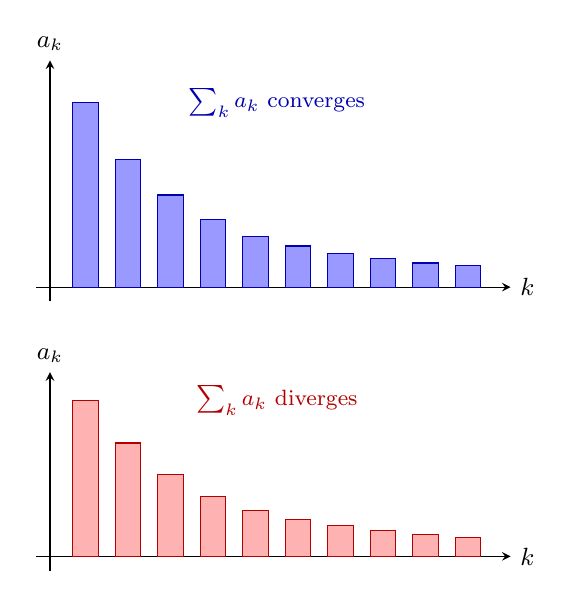
\begin{tikzpicture}[scale=0.9,>=stealth]
  \draw[->] (-0.2,0) -- (6.5,0) node[right, font=\small] {$k$};
  \draw[->] (0,-0.2) -- (0,3.2) node[above, font=\small] {$a_k$};

  \foreach \k/\h in {0.5/2.6, 1.1/1.8, 1.7/1.3, 2.3/0.95, 2.9/0.72, 3.5/0.58, 4.1/0.48, 4.7/0.40, 5.3/0.34, 5.9/0.30} {
    \fill[blue!40] (\k-0.18,0) rectangle (\k+0.18,\h);
    \draw[blue!70!black] (\k-0.18,0) rectangle (\k+0.18,\h);
  }
  \node[font=\footnotesize, blue!70!black] at (3.2,2.6) {$\sum_k a_k$ converges};

  \begin{scope}[yshift=-3.8cm]
    \draw[->] (-0.2,0) -- (6.5,0) node[right, font=\small] {$k$};
    \draw[->] (0,-0.2) -- (0,2.6) node[above, font=\small] {$a_k$};
    \foreach \k/\h in {0.5/2.2, 1.1/1.6, 1.7/1.15, 2.3/0.85, 2.9/0.65, 3.5/0.52, 4.1/0.43, 4.7/0.36, 5.3/0.31, 5.9/0.27} {
      \fill[red!30] (\k-0.18,0) rectangle (\k+0.18,\h);
      \draw[red!70!black] (\k-0.18,0) rectangle (\k+0.18,\h);
    }
    \node[font=\footnotesize, red!70!black] at (3.2,2.2) {$\sum_k a_k$ diverges};
  \end{scope}
\end{tikzpicture}
\caption{Histogram comparison of a convergent (top) and a divergent (bottom) series. When the series converges, the bar heights fall rapidly to zero as $k$ increases; when it diverges, the heights decay too slowly and the partial sums keep growing.}
\label{fig:series_convergence_intuition}
\end{figure}

\begin{remark}[The `speed hierarchy' of series convergence]\label{rem:convergence_speed_hierarchy}
The speed of convergence of a series falls into three levels:
\begin{enumerate}[label=(\roman*)]
  \item \textbf{Geometric rate}: $a_k = O(r^k)$ ($0 < r < 1$), such as $\sum_k r^k$, $\sum_k k^{-k}$.
  \item \textbf{Power-law rate}: $a_k = O(k^{-s})$ ($s > 1$), such as $\sum_k k^{-2}$, $\sum_k k^{-s}$. This is the typical rate of decay of Fourier coefficients in harmonic analysis (the smoothness of Taylor series in the `Functions and Limits' chapter).
  \item \textbf{Logarithmic rate}: $a_k = O(1/(k \log^{1+\varepsilon} k))$, such as $\sum_k 1/(k \log^2 k)$.
\end{enumerate}
The rate of convergence is directly related to the smoothness of the function, the decay of the Fourier coefficients and estimates for the Taylor remainder (Theorem \ref{thm:taylor_lagrange}, \cref{prop:amplitude_series_properties}(v)).
\end{remark}

\section{\texorpdfstring{Taylor Series: Local Derivative Expansion}{Taylor Series}}

\begin{definition}[Taylor Series]\label{def:taylor_series}
Let $f$ be infinitely differentiable in a neighbourhood of $x_0$. The \textbf{Taylor series} of $f$ at $x_0$ is
\[
f(x) \sim \sum_{k=0}^{\infty} \frac{f^{(k)}(x_0)}{k!}(x - x_0)^k.
\]
Its partial sum of the first $n+1$ terms is called the \textbf{Taylor polynomial} $P_n(x)$ of order $n$. If the series converges to $f$ in some neighbourhood of $x_0$, then $f$ is said to be \textbf{real analytic} in that neighbourhood.
\end{definition}

\begin{theorem}[Taylor Formula with Lagrange Remainder]\label{thm:taylor_lagrange}
Let $f$ be $n+1$ times continuously differentiable on $[x_0, x]$ (or $[x, x_0]$) and $n+1$ times differentiable on the open interval. Then there exists $\xi$ between $x_0$ and $x$ such that
\[
f(x) = \sum_{k=0}^{n} \frac{f^{(k)}(x_0)}{k!}(x-x_0)^k + \frac{f^{(n+1)}(\xi)}{(n+1)!}(x-x_0)^{n+1}.
\]
\end{theorem}

\begin{proof}
Write the remainder $R_n(x) = f(x) - P_n(x)$. Define the auxiliary function
\[
F(t) = f(x) - \sum_{k=0}^{n} \frac{f^{(k)}(t)}{k!}(x-t)^k - R_n(x)\cdot\frac{(x-t)^{n+1}}{(x-x_0)^{n+1}}.
\]
Substituting gives $F(x_0) = f(x) - P_n(x) - R_n(x) = 0$, and $F(x) = 0$. By Rolle's theorem there exists $\xi$ with $F'(\xi) = 0$. In the term-by-term differentiation the intermediate terms cancel in pairs, leaving only the first and last:
\[
F'(t) = -\frac{f^{(n+1)}(t)}{n!}(x-t)^n + \frac{(n+1) R_n(x)}{(x-x_0)^{n+1}}(x-t)^n.
\]
Setting $t = \xi$ gives the remainder formula.
\end{proof}

\begin{corollary}[Sufficient Condition for a Taylor Series to Converge to the Function]\label{cor:taylor_analytic}
If there exists a constant $M > 0$ such that the derivatives of $f$ of every order on the interval $I$ satisfy $|f^{(k)}(x)| \le M$ ($x \in I$, $k \ge 0$), then the Taylor series of $f$ at every point of $I$ converges to $f$.
\end{corollary}

\begin{proof}
The Lagrange remainder satisfies
\[
|R_n(x)| \le \frac{M}{(n+1)!}|x - x_0|^{n+1} \to 0 \qquad (n \to \infty).
\]
\end{proof}

\begin{example}[Taylor Series of Elementary Functions]\label{ex:taylor_examples}
\[
e^x = \sum_{k=0}^{\infty} \frac{x^k}{k!}, \qquad
\sin x = \sum_{k=0}^{\infty} \frac{(-1)^k x^{2k+1}}{(2k+1)!}, \qquad
\cos x = \sum_{k=0}^{\infty} \frac{(-1)^k x^{2k}}{(2k)!},
\]
\[
\ln(1+x) = \sum_{k=1}^{\infty} \frac{(-1)^{k+1} x^k}{k} \quad (|x| < 1), \qquad
(1+x)^{\alpha} = \sum_{k=0}^{\infty} \binom{\alpha}{k} x^k \quad (|x| < 1).
\]
\end{example}

\begin{proposition}[Uniqueness of the coefficients of a Taylor expansion]\label{prop:taylor_coefficient_uniqueness}
Suppose $f$ can be expanded in a power series $f(x) = \sum_{k=0}^{\infty} a_k (x-x_0)^k$ in a neighbourhood of $x_0$. Then $a_k = f^{(k)}(x_0)/k!$.
\end{proposition}

\begin{proof}
Differentiate the series term by term $k$ times and evaluate at $x = x_0$. Since a power series may be differentiated term by term inside its circle of convergence (Theorem \ref{thm:uniform_termwise_differentiation}), we obtain $f^{(k)}(x_0) = k!\,a_k$, that is $a_k = f^{(k)}(x_0)/k!$.
\end{proof}

\begin{corollary}[Approximation order of Taylor polynomials]\label{cor:taylor_approximation_order}
Let $f \in C^{n+1}(I)$, $x_0 \in I$. Then the Taylor polynomial $P_n(x)$ satisfies
\[
f(x) - P_n(x) = O(|x - x_0|^{n+1}) \qquad (x \to x_0).
\]
\end{corollary}

\begin{proof}
By the Lagrange remainder formula (Theorem \ref{thm:taylor_lagrange}), $|R_n(x)| \le \frac{M_{n+1}}{(n+1)!}|x-x_0|^{n+1}$, where $M_{n+1} = \sup_{|t-x_0| \le |x-x_0|}|f^{(n+1)}(t)| < \infty$ (since $f^{(n+1)}$ is continuous).
\end{proof}

\begin{figure}[htbp]
\centering
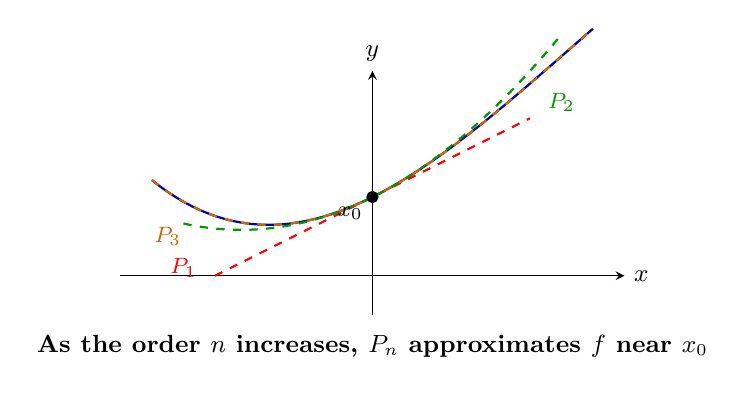
\begin{tikzpicture}[scale=1.0,>=stealth]
  \draw[->] (-3.2,0) -- (3.2,0) node[right, font=\small] {$x$};
  \draw[->] (0,-0.5) -- (0,2.6) node[above, font=\small] {$y$};

  \draw[thick, blue!70!black, domain=-2.8:2.8, samples=120]
    plot (\x, {1.0 + 0.5*\x + 0.15*\x*\x - 0.02*\x*\x*\x});

  \draw[thick, red, dashed, domain=-2.0:2.0, samples=80]
    plot (\x, {1.0 + 0.5*\x});
  \node[red, font=\footnotesize] at (-2.4,0.1) {$P_1$};

  \draw[thick, green!60!black, dashed, domain=-2.4:2.4, samples=80]
    plot (\x, {1.0 + 0.5*\x + 0.15*\x*\x});
  \node[green!60!black, font=\footnotesize] at (2.4,2.2) {$P_2$};

  \draw[thick, orange!80!black, dashed, domain=-2.8:2.8, samples=100]
    plot (\x, {1.0 + 0.5*\x + 0.15*\x*\x - 0.02*\x*\x*\x});
  \node[orange!80!black, font=\footnotesize] at (-2.6,0.5) {$P_3$};

  \filldraw[black] (0,1.0) circle (2pt);
  \node[font=\footnotesize, below left] at (0,1.0) {$x_0$};

  \node[font=\small\bfseries] at (0,-0.9) {As the order $n$ increases, $P_n$ approximates $f$ near $x_0$};
\end{tikzpicture}
\caption{Successive approximation by Taylor polynomials. $P_1$ (linear) approximates $f$ near $x_0$; $P_2$ (quadratic) adds a curvature correction; $P_3$ (cubic) corrects it further. The higher the order, the wider the interval of approximation.}
\label{fig:taylor_approximation}
\end{figure}

\begin{remark}[The duality between Taylor and Fourier expansions]\label{rem:taylor_fourier_duality}
The Taylor expansion and the Fourier expansion form a \textbf{local--global} duality:
\begin{center}
\begin{tabular}{@{}p{3.2cm}p{4.2cm}p{4.2cm}@{}}
\toprule
 & Taylor expansion & Fourier expansion \\
\midrule
Centre of expansion & a single point $x_0$ & the periodic interval $[0,T]$ \\
Source of coefficients & the derivative $f^{(k)}(x_0)$ & the integral $c_n = \frac{1}{T}\int_0^T f(t) e^{-i\omega_n t} dt$ \\
Type of information & direction (local derivatives) & trend (global integrals) \\
Convergence condition & real analytic & $L^2$ integrable + Dirichlet conditions \\
Basis functions & $(x-x_0)^k$ (polynomials) & $e^{i\omega_n t}$ (complex exponentials) \\
\bottomrule
\end{tabular}
\end{center}
This duality is the manifestation, at the level of function expansions, of the direction--trend duality of the `Scalars and Vectors' chapter (Remark \ref{rem:fourier_coefficient_duality}).
\end{remark}

\section{\texorpdfstring{Laurent Series: Complex Expansion with Negative Powers}{Laurent Series}}

\begin{definition}[Laurent Series]\label{def:laurent_series}
Let $z_0 \in \mathbb{C}$. A series of the form
\[
f(z) = \sum_{n=-\infty}^{\infty} a_n (z - z_0)^n
\]
is called a \textbf{Laurent series} centred at $z_0$. The positive-power part converges in the disc $|z-z_0| < R$, whilst the negative-power part, after the change of variable $w = 1/(z-z_0)$, converges on $|z-z_0| > r$; the common domain of convergence is the annulus $r < |z-z_0| < R$.
\end{definition}

\begin{lemma}[Uniqueness of Laurent Coefficients]\label{lem:laurent_uniqueness}
If $\sum_{n} a_n (z-z_0)^n = \sum_{n} b_n (z-z_0)^n$ on some annulus, then $a_n = b_n$ for all $n \in \mathbb{Z}$.
\end{lemma}

\begin{proof}
Let $d_n = a_n - b_n$. For any $m \in \mathbb{Z}$, multiply the identity by $(z-z_0)^{-m-1}$ and integrate along a circle around $z_0$. From
\[
\oint_\gamma (z-z_0)^{n-m-1}\,dz = 2\pi i\, \delta_{nm},
\]
we obtain $d_m \cdot 2\pi i = 0$, hence $d_m = 0$.
\end{proof}

\begin{theorem}[Laurent Expansion Theorem]\label{thm:laurent_expansion}
Let $f$ be analytic in the annulus $r < |z - z_0| < R$. Then $f$ can be expanded uniquely as a Laurent series in that annulus, with coefficients
\[
a_n = \frac{1}{2\pi i} \oint_{\gamma} \frac{f(\zeta)}{(\zeta - z_0)^{n+1}}\, d\zeta, \qquad n \in \mathbb{Z},
\]
where $\gamma$ is any positively oriented closed curve in the annulus surrounding $z_0$.
\end{theorem}

\begin{proof}
By the Cauchy integral formula, for any point $z$ in the annulus and two concentric circles $\gamma_1, \gamma_2$,
\[
f(z) = \frac{1}{2\pi i}\oint_{\gamma_1} \frac{f(\zeta)}{\zeta - z}\,d\zeta - \frac{1}{2\pi i}\oint_{\gamma_2} \frac{f(\zeta)}{\zeta - z}\,d\zeta.
\]
Expanding on $\gamma_1$ by the geometric series gives the positive-power part; a similar expansion on $\gamma_2$ gives the negative-power part. Uniqueness is given by Lemma \ref{lem:laurent_uniqueness}.
\end{proof}

\begin{proposition}[Laurent Expansion of Rotationally Periodic Functions]\label{prop:laurent_rotation_period}
If $f$ satisfies the rotational periodicity $f(e^{i\theta} z) = f(z)$ (group with periodic orbits $C_m$, that is $\theta = 2\pi/m$), then its Laurent series centred at $0$ contains only terms with $n \equiv 0 \pmod{m}$.
\end{proposition}

\begin{proof}
Substituting $z \mapsto e^{i\theta} z$ and using uniqueness of coefficients gives $a_n (e^{in\theta} - 1) = 0$. When $e^{i\theta}$ is a primitive $m$-th root of unity, $e^{in\theta} = 1 \iff m \mid n$.
\end{proof}

\begin{example}[Laurent Expansion of $e^{1/z}$]\label{ex:laurent_example}
\[
e^{1/z} = \sum_{n=0}^{\infty} \frac{z^{-n}}{n!}, \qquad |z| > 0.
\]
\end{example}

\begin{proposition}[Classification of singularities and the principal part of a Laurent series]\label{prop:laurent_singularity}
Let $f$ be analytic on $0 < |z-z_0| < R$, with Laurent expansion $f(z) = \sum_{n=-\infty}^{\infty} a_n (z-z_0)^n$. Calling
\[
\text{principal part} = \sum_{n=1}^{\infty} a_{-n} (z-z_0)^{-n}
\]
the principal part of the Laurent expansion, we have:
\begin{enumerate}[label=(\roman*)]
  \item removable singularity $\iff$ the principal part is zero;
  \item pole of order $m$ $\iff$ the principal part is a non-zero finite sum whose highest negative power is $m$;
  \item essential singularity $\iff$ the principal part has infinitely many terms.
\end{enumerate}
\end{proposition}

\begin{proof}
Each item follows directly from the definition of the negative-power part of the Laurent expansion.
\end{proof}

\begin{example}[Laurent expansions of the three types of singularity compared]\label{ex:three_singularity_types}
\begin{enumerate}[label=(\roman*)]
  \item \textbf{Removable singularity}: $f(z) = \frac{\sin z}{z}$, whose Laurent expansion at $z_0 = 0$ is $1 - z^2/6 + \cdots$, with principal part zero.
  \item \textbf{Pole}: $f(z) = \frac{1}{z^2(z-1)}$, whose principal part at $z_0 = 0$ is $-1 - z - z^2$, so it is a pole of order $2$.
  \item \textbf{Essential singularity}: $f(z) = e^{1/z}$, whose principal part at $z_0 = 0$ is $\sum_{n=1}^{\infty} z^{-n}/n!$, with infinitely many terms.
\end{enumerate}
\end{example}

\begin{theorem}[Duality between the residue theorem and Fourier coefficients]\label{thm:residue_fourier_duality}
Let $f$ be analytic in the annulus $r < |z - z_0| < R$, with Laurent expansion $f(z) = \sum_{n \in \mathbb{Z}} a_n (z-z_0)^n$. Then $a_n$ is represented by the residue as
\[
a_n = \operatorname{Res}\!\left(\frac{f(z)}{(z-z_0)^{n+1}}, z_0\right).
\]
In particular, $a_{-1} = \operatorname{Res}(f, z_0)$ is precisely the coefficient of $(z-z_0)^{-1}$ in the Laurent expansion.
\end{theorem}

\begin{proof}
It follows by directly comparing the Laurent coefficient formula (Theorem \ref{thm:laurent_expansion}) with the definition of the residue (Definition \ref{def:residue} of the `Differential Equations and Analysis' chapter).
\end{proof}

\begin{figure}[htbp]
\centering
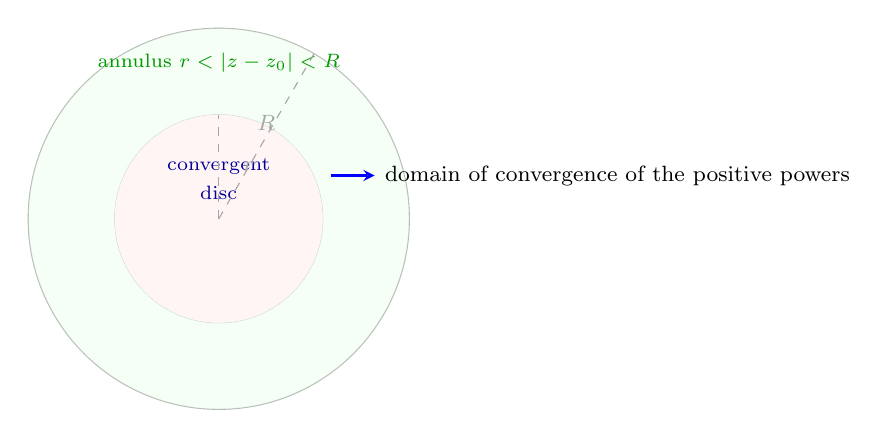
\begin{tikzpicture}[scale=1.1,>=stealth]
  \draw[gray!60, thin] (0,0) circle (2.2);
  \draw[gray!60, thin] (0,0) circle (1.2);
  \filldraw[red!70!black] (0,0) circle (2.5pt);
  \node[red!70!black, font=\footnotesize, below left=1pt] at (0,0) {$z_0$};

  \fill[blue!10, opacity=0.5] (0,0) circle (1.2);
  \fill[green!10, opacity=0.4] (0,0) circle (2.2);
  \fill[white, opacity=1.0] (0,0) circle (1.2);
  \fill[red!5, opacity=0.7] (0,0) circle (1.2);

  \node[font=\scriptsize, blue!60!black] at (0,0.6) {convergent};
  \node[font=\scriptsize, blue!60!black] at (0,0.3) {disc};
  \node[font=\scriptsize, green!60!black] at (0,1.8) {annulus $r < |z - z_0| < R$};

  \draw[->, thick, blue] (1.3,0.5) -- (1.8,0.5) node[right, font=\footnotesize, black] {domain of convergence of the positive powers};

  \draw[gray!70, dashed] (0,0) -- (0,1.2);
  \node[gray!70, font=\footnotesize] at (0.35,0.6) {$r$};
  \draw[gray!70, dashed] (0,0) -- ({cos(60)*2.2}, {sin(60)*2.2});
  \node[gray!70, font=\footnotesize] at ({cos(60)*1.1}, {sin(60)*1.1 + 0.15}) {$R$};
\end{tikzpicture}
\caption{The annulus of convergence of a Laurent series. The positive-power part converges in the disc centred at $z_0$, whilst the negative-power part converges in the region near the point at infinity; their common domain of convergence is the annulus $r < |z - z_0| < R$.}
\label{fig:laurent_annulus}
\end{figure}

\section{\texorpdfstring{Fourier Series: Global Decomposition on the Harmonic Lattice}{Fourier Series}}

\begin{definition}[Fourier Series (Complex and Real Forms)]\label{def:fourier_series_foundations}
Let $f$ have period $T$ and be integrable on $[0,T]$. The \textbf{Fourier series} of $f$ (complex form) is
\[
f(t) \sim \sum_{n=-\infty}^{\infty} c_n e^{i 2\pi n t / T}, \qquad
c_n = \frac{1}{T}\int_0^T f(t) e^{-i 2\pi n t / T}\,dt.
\]
The real form is
\[
f(t) \sim \frac{a_0}{2} + \sum_{n=1}^{\infty} \Big( a_n \cos\frac{2\pi n t}{T} + b_n \sin\frac{2\pi n t}{T} \Big),
\]
where $a_n = c_n + c_{-n}$, $b_n = i(c_n - c_{-n})$.
\end{definition}

\begin{proposition}[Orthogonality of the Fourier Basis]\label{prop:fourier_orthogonality}
The system of functions $\{e^{i 2\pi n t / T}\}_{n \in \mathbb{Z}}$ is orthogonal in $L^2([0,T])$:
\[
\frac{1}{T}\int_0^T e^{i 2\pi (n-m) t / T}\,dt = \delta_{nm}.
\]
\end{proposition}

\begin{proof}
When $n = m$ the integrand is $1$; when $n \neq m$ the integral becomes $\frac{T}{2\pi i (n-m)}(e^{i 2\pi (n-m)} - 1) = 0$.
\end{proof}

\begin{theorem}[Parseval's Identity (Fourier Series)]\label{thm:parseval_fourier_classical}
Let $f \in L^2([0,T])$ with Fourier coefficients $c_n$. Then
\[
\frac{1}{T}\int_0^T |f(t)|^2\,dt = \sum_{n=-\infty}^{\infty} |c_n|^2.
\]
\end{theorem}

\begin{proof}
For trigonometric polynomials it holds directly by orthogonality (Proposition \ref{prop:fourier_orthogonality}); for general $L^2$ functions it follows from the completeness of the Fourier basis in $L^2$ by approximation.
\end{proof}

\begin{example}[Fourier Series of a Square Wave]\label{ex:fourier_square_wave}
Let $f$ have period $T$, take the value $1$ on $[0, T/2)$ and the value $-1$ on $[T/2, T)$. Its Fourier series is
\[
f(t) \sim \frac{4}{\pi} \sum_{k=0}^{\infty} \frac{1}{2k+1} \sin\frac{2\pi (2k+1) t}{T}.
\]
\end{example}

\begin{theorem}[Dirichlet convergence theorem]\label{thm:dirichlet_convergence}
Let $f$ have period $T$ and be piecewise $C^1$ on $[0,T]$. Then the Fourier series of $f$ converges at every point $t$ to
\[
\frac{f(t^+) + f(t^-)}{2},
\]
where $f(t^+)$ and $f(t^-)$ are the right-hand and left-hand limits of $f$ at $t$ respectively. In particular, at every point where $f$ is continuous, the Fourier series converges to $f(t)$.
\end{theorem}

\begin{proof}[Sketch of proof]
Write the Fourier partial sum of $f$ as a convolution with the Dirichlet kernel $D_N$:
\[
S_N f(t) = \frac{1}{T}\int_0^T f(t - \tau) D_N(\tau)\,d\tau.
\]
Using the properties of the Dirichlet kernel: $\frac{1}{T}\int_0^T D_N(\tau)\,d\tau = 1$, and $D_N$ oscillates with alternating signs away from $0$, so that the contributions cancel (the Riemann--Lebesgue lemma). The piecewise $C^1$ condition guarantees that the local one-sided behaviour of $f$ near $t$ can be controlled by a first-order Taylor expansion, so that $S_N f(t) \to [f(t^+) + f(t^-)]/2$. For a rigorous proof see Zygmund, \textit{Trigonometric Series}, 3rd ed., Cambridge Univ. Press, 2002, \S{}II.4.
\end{proof}

\begin{corollary}[Pointwise convergence at points of continuity]\label{cor:fourier_continuity}
If $f$ is continuous at $t$, then $f(t^+) = f(t^-) = f(t)$ and the Fourier series converges to $f(t)$ at $t$.
\end{corollary}

\begin{example}[The Gibbs phenomenon]\label{ex:gibbs_phenomenon}
The Fourier partial sums $S_N f$ of the square wave $f(t) = \operatorname{sgn}(\sin t)$ exhibit an \textbf{overshoot} of about $9\%$ near the jump point $t = 0$, and the magnitude of the overshoot does not decay as $N \to \infty$. This phenomenon is called the \textbf{Gibbs phenomenon}; it shows that uniform convergence of the Fourier series fails near a jump point (pointwise convergence still holds, by Theorem \ref{thm:dirichlet_convergence}). In digital signal processing the Gibbs phenomenon is equivalent to the ringing effect of an `ideal low-pass filter'.
\end{example}

\begin{theorem}[The Fej\'er kernel and uniform convergence]\label{thm:fejer_uniform}
Let $f$ have period $T$ and be continuous. Define the Fej\'er means
\[
\sigma_N f(t) = \frac{1}{N+1}\sum_{k=0}^{N} S_k f(t),
\]
where $S_k f$ is the $k$-th Fourier partial sum. Then $\sigma_N f$ converges uniformly to $f$ on $\mathbb{R}$.
\end{theorem}

\begin{proof}[Sketch of proof]
The Fej\'er mean can be written as a convolution with the Fej\'er kernel $\sigma_N f(t) = \frac{1}{T}\int_0^T f(t-\tau) F_N(\tau)\,d\tau$, where
\[
F_N(\tau) = \frac{1}{N+1}\left(\frac{\sin((N+1)\tau/2)}{\sin(\tau/2)}\right)^2.
\]
The Fej\'er kernel is a \textbf{good kernel}: non-negative, of integral $1$, and tending to zero uniformly away from $\tau \neq 0$. Hence for a continuous periodic function $f$, the uniform approximation property of good kernels gives $\sigma_N f \to f$ uniformly. For a rigorous proof see Zygmund, \textit{Trigonometric Series}, 3rd ed., Cambridge Univ. Press, 2002, \S{}III.1.
\end{proof}

\begin{figure}[htbp]
\centering
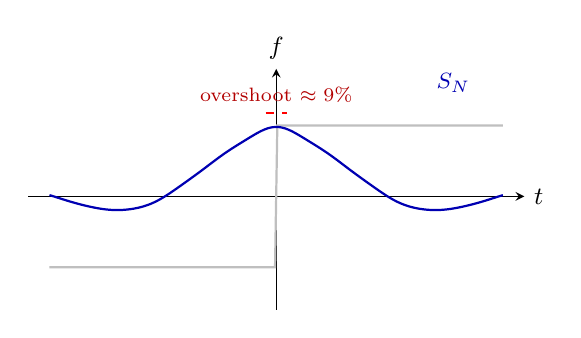
\begin{tikzpicture}[scale=0.9,>=stealth]
  \draw[->] (-3.5,0) -- (3.5,0) node[right, font=\small] {$t$};
  \draw[->] (0,-1.6) -- (0,1.8) node[above, font=\small] {$f$};

  \draw[thick, gray!50, domain=-3.2:3.2, samples=200]
    plot (\x, {(\x>0?1:-1)});

  \draw[thick, blue!70!black, domain=-3.2:3.2, samples=200]
    plot (\x, {0.9*sin(deg(2*\x))/(2*\x) + 0.05*sin(deg(6*\x))/(6*\x) + 0.03*sin(deg(10*\x))/(10*\x)});
  \node[blue!70!black, font=\footnotesize] at (2.5,1.6) {$S_N$};

  \draw[red, thick, dashed] (-0.15,1.18) -- (0.15,1.18);
  \node[red!70!black, font=\scriptsize, above] at (0,1.18) {overshoot $\approx 9\%$};
\end{tikzpicture}
\caption{The Gibbs phenomenon. The Fourier partial sum $S_N$ (blue) of the square wave (grey) exhibits an overshoot (red dashed line) near the jump point $t = 0$; the magnitude of the overshoot is about $9\%$ of the jump and does not disappear as $N$ increases.}
\label{fig:gibbs}
\end{figure}

\begin{property}[Preservation under integration for Fourier series]\label{prop:fourier_integration_preservation}
Let $f$ have period $T$, be integrable on $[0,T]$ and have zero mean (that is, $c_0 = 0$). Then the indefinite integral $F(t) = \int_0^t f(\tau)\,d\tau$ has period $T$, and its Fourier coefficients are $C_n = c_n / (i\omega_n)$ ($n \neq 0$).
\end{property}

\begin{proof}
From $c_0 = 0$ we obtain $F(T) = \int_0^T f = T c_0 = 0$, so $F$ has period $T$. The Fourier coefficients of $F$ are
\[
C_n = \frac{1}{T}\int_0^T F(t) e^{-i\omega_n t}\,dt = \frac{1}{T} \cdot \frac{1}{i\omega_n}\left[ F(t) e^{-i\omega_n t} \Big|_0^T + \int_0^T f(t) e^{-i\omega_n t}\,dt \right] = \frac{c_n}{i\omega_n}.
\]
(Integration by parts; the boundary terms vanish by periodicity.)
\end{proof}

\begin{remark}[Three modes of convergence of Fourier series]\label{rem:fourier_convergence_modes}
The Fourier series has three modes of convergence, each corresponding to different conditions and conclusions:
\begin{center}
\begin{tabular}{@{}p{2.5cm}p{4.0cm}p{5.0cm}@{}}
\toprule
Mode of convergence & Condition & Conclusion \\
\midrule
Pointwise convergence & $f$ piecewise $C^1$ & $S_N f(t) \to [f(t^+)+f(t^-)]/2$ (Theorem \ref{thm:dirichlet_convergence}) \\
Uniform convergence & $f$ continuous + $\sum |c_n| < \infty$ & $S_N f \to f$ uniformly (Fej\'er means, Theorem \ref{thm:fejer_uniform}) \\
$L^2$ convergence & $f \in L^2[0,T]$ & $\|S_N f - f\|_2 \to 0$ (Parseval + completeness) \\
\bottomrule
\end{tabular}
\end{center}
The three modes do not imply one another: uniform convergence $\Rightarrow$ pointwise convergence, but not conversely (the Gibbs phenomenon); $L^2$ convergence and pointwise convergence do not imply one another.
\end{remark}

\begin{remark}[Direction--Trend Duality of Fourier Coefficients]\label{rem:fourier_coefficient_duality}
The Fourier coefficients $c_n$ are given by integrals (trend information) and the Taylor coefficients by derivatives (direction information); the two form a direction--trend duality. The problems of pointwise and uniform convergence of Fourier series can be handled by tools such as the Dirichlet kernel, the Gibbs phenomenon and Fej\'er-kernel smoothing; we shall not develop them in this chapter.
\end{remark}

\section{\texorpdfstring{He Tu Complex Functions: The $\mathbb{Z}_2 \times \mathbb{Z}_5$ Decomposition of Period 10}{He Tu Complex Functions}}
\label{sec:hetu_function}

This section establishes the \textbf{He Tu complex function}---a complex function of period $10$. Its mathematical core is this: in the Fourier decomposition of period $10$ there automatically appears the algebraic grading $\mathbb{Z}_{10} \cong \mathbb{Z}_2 \times \mathbb{Z}_5$, in which the $\mathbb{Z}_5$ component corresponds to a fivefold cycle and the $\mathbb{Z}_2$ component to a twofold alternation. This grading is a purely algebraic fact about the Fourier expansion of discrete periodic functions and does not depend on any cultural interpretation.

\begin{definition}[The $\mathbb{Z}_5$ Projection on $\mathbb{Z}_{10}$]\label{def:hetu_mapping}
Define the group homomorphism $\varphi: \mathbb{Z}_{10} \to \mathbb{Z}_5$ by
\[
\varphi(n) := n \bmod 5, \qquad n \in \mathbb{Z}_{10} = \{0, 1, \dots, 9\},
\]
with the convention that the remainder $0$ corresponds to the label `earth'. Specifically:
\[
\begin{array}{c|ccccc}
\varphi(n) & 0 & 1 & 2 & 3 & 4 \\
\hline
\text{Label} & \text{earth} & \text{water} & \text{fire} & \text{wood} & \text{metal} \\
\text{Numbers} & 5, 10 & 1, 6 & 2, 7 & 3, 8 & 4, 9
\end{array}
\]
There is also a $\mathbb{Z}_2$ component, given by the parity of $n$. The kernel of $\varphi$ is
\[
\ker \varphi = \{0, 5\} \cong \mathbb{Z}_2.
\]
\end{definition}

\begin{definition}[He Tu Complex Function]\label{def:hetu_function}
Let $f: \mathbb{C} \to \mathbb{C}$ satisfy the periodicity condition
\[
f(z + 10) = f(z), \qquad \forall z \in \mathbb{C}.
\]
Then $f$ is called a \textbf{He Tu complex function}. Its Fourier expansion is
\[
f(z) = \sum_{n \in \mathbb{Z}} c_n\, e^{2\pi i n z / 10}, \qquad c_n = \frac{1}{10}\int_0^{10} f(t)\, e^{-2\pi i n t / 10}\, dt.
\]
\end{definition}

\begin{theorem}[He Tu Fourier Decomposition---$\mathbb{Z}_2 \times \mathbb{Z}_5$ Grading]\label{thm:hetu_fourier_decomposition}
Let $f$ be a He Tu complex function whose Fourier expansion converges uniformly on $\mathbb{C}$. Then $f$ decomposes uniquely as
\[
\boxed{\,f(z) = \sum_{k=0}^{4} \Bigl( c_k + c_{k+5}\, e^{\pi i z} \Bigr)\, e^{2\pi i k z / 10}\,,}
\]
where $c_k$ are the Fourier coefficients and $e^{\pi i z}$ is the $\mathbb{Z}_2$ factor of period $2$. This decomposition is the explicit form of $\mathbb{Z}_{10} \cong \mathbb{Z}_2 \times \mathbb{Z}_5$ in the Fourier expansion.
\end{theorem}

\begin{proof}
Using $\mathbb{Z}_{10} \cong \mathbb{Z}_2 \times \mathbb{Z}_5$, write the integer index $n \in \mathbb{Z}$ uniquely as
\[
n = 5\varepsilon + k, \qquad \varepsilon \in \{0, 1\}, \quad k \in \{0, 1, 2, 3, 4\}.
\]
Substituting into the Fourier basis functions:
\[
e^{2\pi i n z / 10} = e^{2\pi i (5\varepsilon + k) z / 10} = e^{\pi i \varepsilon z} \cdot e^{2\pi i k z / 10}.
\]
Decompose the sum over $n$ according to $\varepsilon$:
\[
f(z) = \sum_{\varepsilon \in \{0,1\}} \sum_{k=0}^{4} c_{5\varepsilon+k}\, e^{\pi i \varepsilon z}\, e^{2\pi i k z / 10}.
\]
Extracting the $\varepsilon = 0$ and $\varepsilon = 1$ terms and collecting like terms $e^{2\pi i k z / 10}$:
\[
f(z) = \sum_{k=0}^{4} \Bigl( c_k + c_{k+5}\, e^{\pi i z} \Bigr)\, e^{2\pi i k z / 10}.
\]
Uniqueness is guaranteed by the uniqueness of the Fourier coefficients (Bohr means) and the bijection $n \mapsto (5\varepsilon + k)$.
\end{proof}

\begin{definition}[The $\mathbb{Z}_5$ Components]\label{def:hetu_five_components}
In the above decomposition, the function
\[
f_k(z) := \Bigl( c_k + c_{k+5}\, e^{\pi i z} \Bigr)\, e^{2\pi i k z / 10}, \qquad k = 0, 1, 2, 3, 4
\]
is called the \textbf{$k$-th $\mathbb{Z}_5$ component} of $f$. According to the labels of Definition \ref{def:hetu_mapping}, the five components correspond in order to: earth, water, fire, wood and metal. Each component consists of two parts: $c_k\, e^{2\pi i k z / 10}$ (the $\varepsilon = 0$ component) and $c_{k+5}\, e^{\pi i z} e^{2\pi i k z / 10}$ (the $\varepsilon = 1$ component).
\end{definition}

\begin{proposition}[Period Structure of the $\mathbb{Z}_5$ Components]\label{prop:hetu_five_periods}
The fundamental periods of the five $\mathbb{Z}_5$ components $f_0, f_1, f_2, f_3, f_4$ are respectively:
\[
\begin{array}{c|ccccc}
k & 0 & 1 & 2 & 3 & 4 \\
\hline
\text{Label} & \text{earth} & \text{water} & \text{fire} & \text{wood} & \text{metal} \\
\text{Fundamental period} & 1 & 10 & 5 & 10 & 5
\end{array}
\]
That is: $f_0$ contains only a constant term; $f_1, f_3$ are components of period $10$; $f_2, f_4$ are components of period $5$.
\end{proposition}

\begin{proof}
The fundamental frequency of the component $f_k$ is $e^{2\pi i k z / 10}$, whose fundamental period is $10/\gcd(k, 10)$. Substituting one by one:
\begin{itemize}
    \item $k = 0$: $10/\gcd(0,10) = 1$ (with the convention $\gcd(0,10) = 10$), so the fundamental-frequency part of $f_0$ is constant.
    \item $k = 1$: $10/\gcd(1,10) = 10$.
    \item $k = 2$: $10/\gcd(2,10) = 5$.
    \item $k = 3$: $10/\gcd(3,10) = 10$.
    \item $k = 4$: $10/\gcd(4,10) = 5$.
\end{itemize}
The $\mathbb{Z}_2$ factor $e^{\pi i z}$ has period $2$ and does not change the above period structure (because $2 \mid 10$).
\end{proof}

\begin{proposition}[Half-Period Translation of He Tu Complex Functions]\label{prop:hetu_yin_yang_flip}
Let $f$ be a He Tu complex function and $f = \sum_{k=0}^{4} f_k$ its $\mathbb{Z}_5$ decomposition. Then the half-period translation $z \mapsto z + 5$ gives
\[
f(z + 5) = \sum_{k=0}^{4} \Bigl( (-1)^k c_k + (-1)^k c_{k+5}\, e^{\pi i z} \Bigr)\, e^{2\pi i k z / 10},
\]
that is, each $\mathbb{Z}_5$ component acquires a factor $(-1)^k$: even components ($k = 0, 2, 4$) are unchanged, whilst odd components ($k = 1, 3$) change sign as a whole.
\end{proposition}

\begin{proof}
By Theorem \ref{thm:hetu_fourier_decomposition}, $f(z+5) = \sum_k (c_k + c_{k+5} e^{\pi i (z+5)}) e^{2\pi i k (z+5)/10}$. Computing separately:
\[
e^{\pi i (z+5)} = e^{\pi i z} e^{5\pi i} = -e^{\pi i z},\qquad
e^{2\pi i k (z+5)/10} = e^{2\pi i k z / 10}\, e^{\pi i k} = (-1)^k\, e^{2\pi i k z / 10}.
\]
Substituting gives the result.
\end{proof}

\begin{definition}[$\mathbb{Z}_{10}$ Phase Operators]\label{def:hetu_phase_operator}
The \textbf{$\mathbb{Z}_{10}$ phase operator} is defined by
\[
\mathcal{O}_n^{(10)} := e^{2\pi i n / 10}, \qquad n = 0, 1, \dots, 9.
\]
Under the decomposition $\mathbb{Z}_{10} \cong \mathbb{Z}_2 \times \mathbb{Z}_5$, the phase operator can be written as
\[
\mathcal{O}_{5\varepsilon + k}^{(10)} = (-1)^\varepsilon\, e^{2\pi i k / 10}, \qquad \varepsilon \in \{0, 1\}, \; k \in \{0, 1, 2, 3, 4\},
\]
that is, each phase operator is the product of the $\mathbb{Z}_2$ sign $(-1)^\varepsilon$ and the $\mathbb{Z}_5$ phase $e^{2\pi i k / 10}$.
\end{definition}

\begin{proposition}[Direct Product Decomposition of the $\mathbb{Z}_{10}$ Phase Operator Group]\label{prop:hetu_phase_group}
The group of $\mathbb{Z}_{10}$ phase operators $\{\mathcal{O}_n^{(10)}\}_{n=0}^{9}$ is isomorphic to
\[
C_{10} \cong C_2 \times C_5,
\]
where $C_2 = \{+1, -1\}$ corresponds to the $\mathbb{Z}_2$ component and $C_5 = \{e^{2\pi i k/5}\}_{k=0}^{4}$ to the $\mathbb{Z}_5$ component. The generator $\mathcal{O}_1^{(10)} = e^{\pi i / 5}$ corresponds under the decomposition to $(1, e^{2\pi i / 10})$ and has order $10 = \operatorname{lcm}(2, 5)$.
\end{proposition}

\begin{proof}
The map $\mathcal{O}_{5\varepsilon + k}^{(10)} \mapsto ((-1)^\varepsilon, e^{2\pi i k / 10})$ is a group isomorphism: from
\[
\mathcal{O}_{5\varepsilon_1 + k_1}^{(10)} \cdot \mathcal{O}_{5\varepsilon_2 + k_2}^{(10)} = \mathcal{O}_{5(\varepsilon_1 + \varepsilon_2) + (k_1 + k_2)}^{(10)},
\]
the right-hand side corresponds to $((-1)^{\varepsilon_1 + \varepsilon_2}, e^{2\pi i (k_1 + k_2)/10})$, exactly the product of the two components. That the isomorphism is bijective is guaranteed by $\mathbb{Z}_{10} \cong \mathbb{Z}_2 \times \mathbb{Z}_5$. The order of the generator $= \operatorname{lcm}(2, 5) = 10$.
\end{proof}

\begin{theorem}[DFT Diagonalisation of He Tu Circulant Matrices]\label{thm:hetu_circulant}
Let $\mathbf{C}$ be a $10 \times 10$ circulant matrix whose first row has generators $(h_0, h_1, \dots, h_9)$, with $h_n$ assigned $\mathbb{Z}_2 \times \mathbb{Z}_5$ labels according to Definition \ref{def:hetu_mapping}. Then $\mathbf{C}$ is unitarily diagonalised by the DFT matrix $\mathbf{F}_{10}$:
\[
\mathbf{C} = \mathbf{F}_{10}^*\, \operatorname{diag}(\hat{h}_0, \hat{h}_1, \dots, \hat{h}_9)\, \mathbf{F}_{10}, \qquad
\hat{h}_n = \sum_{j=0}^{9} h_j\, e^{-2\pi i j n / 10}.
\]
Furthermore, the eigenvalues $\hat{h}_n$ are graded according to $\mathbb{Z}_{10} \cong \mathbb{Z}_2 \times \mathbb{Z}_5$: the five eigenvalues $(\hat{h}_0, \hat{h}_1, \hat{h}_2, \hat{h}_3, \hat{h}_4)$ corresponding to $\varepsilon = 0$ belong to the $C_5$ component, and the five eigenvalues $(\hat{h}_5, \hat{h}_6, \hat{h}_7, \hat{h}_8, \hat{h}_9)$ corresponding to $\varepsilon = 1$ belong to the $\mathbb{Z}_2$ translation component.
\end{theorem}

\begin{proof}
By the DFT diagonalisation of circulant matrices (a standard result), $\mathbf{C} = \mathbf{F}_{10}^* \operatorname{diag}(\hat{h}) \mathbf{F}_{10}$. The eigenvalues $\hat{h}_n$ split into two groups according to $n = 5\varepsilon + k$: $n \in \{0,1,2,3,4\}$ corresponds to $\varepsilon = 0$, and $n \in \{5,6,7,8,9\}$ to $\varepsilon = 1$. Since $\hat{h}_{n+5} = \sum_j h_j e^{-2\pi i j (n+5)/10} = \sum_j h_j (-1)^j e^{-2\pi i j n/10}$, that is, $\hat{h}_{n+5}$ is determined by the parity weighting of the $h_j$ and is independent of $\hat{h}_n$.
\end{proof}

\begin{example}[Concrete Decomposition of a He Tu Complex Function]\label{ex:hetu_concrete}
Take $f(z) = 3 + 2 e^{\pi i z / 5} + e^{\pi i z} + 5 e^{3\pi i z / 5} + 4 e^{2\pi i z}$. This function has period $10$; write it in the standard form of Theorem \ref{thm:hetu_fourier_decomposition}.

First arrange the Fourier coefficients in order of $n$: $c_0 = 3$, $c_1 = 2$, $c_5 = 1$, $c_3 = 5$, $c_4 = 4$, with the remaining $c_n = 0$. Decompose according to $n = 5\varepsilon + k$:
\[
f(z) = \underbrace{3}_{n=0} + \underbrace{2 e^{\pi i z / 5}}_{n=1} + \underbrace{5 e^{3\pi i z / 5}}_{n=3} + \underbrace{4 e^{2\pi i z}}_{n=4} + \underbrace{e^{\pi i z}}_{n=5}.
\]
The $(\varepsilon, k)$ label of each term and its $\mathbb{Z}_2 \times \mathbb{Z}_5$ membership are as in the following table:
\[
\begin{array}{c|ccccc}
n & 0 & 1 & 3 & 4 & 5 \\
\hline
(\varepsilon, k) & (0, 0) & (0, 1) & (0, 3) & (0, 4) & (1, 0) \\
\text{Label} & \text{earth} & \text{water} & \text{wood} & \text{metal} & \text{earth} \\
\text{Component} & C_5 & C_5 & C_5 & C_5 & \mathbb{Z}_2
\end{array}
\]
Collecting like $\mathbb{Z}_5$ components:
\[
f_0 = 3 + e^{\pi i z}, \quad f_1 = 2 e^{\pi i z/5}, \quad f_2 = 0, \quad f_3 = 5 e^{3\pi i z/5}, \quad f_4 = 4 e^{2\pi i z}.
\]
By Proposition \ref{prop:hetu_five_periods}, $f_0$ contains a constant term (period $1$); $f_1, f_3$ have period $10$; $f_4$ has period $5$.
\end{example}

\begin{remark}[Algebraic Meaning of the He Tu Structure]\label{rem:hetu_algebraic_meaning}
The mathematical content of the He Tu complex function lies in the Fourier grading $\mathbb{Z}_{10} \cong \mathbb{Z}_2 \times \mathbb{Z}_5$:
\begin{itemize}
    \item the $\mathbb{Z}_5$ component corresponds to the fivefold cycle of the Fourier mode $k \in \{0,1,2,3,4\}$;
    \item the $\mathbb{Z}_2$ component corresponds to the parity of the Fourier mode $n$, that is, a twofold alternation;
    \item the half-period translation $z \mapsto z + 5$ changes the sign of the components with odd $k$ as a whole (Proposition \ref{prop:hetu_yin_yang_flip}).
\end{itemize}
The He Tu map $\varphi: \mathbb{Z}_{10} \to \mathbb{Z}_5$ is a group homomorphism whose kernel is $\{0, 5\} \cong \mathbb{Z}_2$. This gives the grading a rigorous algebraic realisation in the Fourier expansion---not an imposed encoding, but an algebraic structure that appears automatically in the Fourier decomposition of period $10$.
\end{remark}

\section{\texorpdfstring{Amplitude Series}{Amplitude Series}}

This section discusses the form of series with zero phase and period $2\pi$. It is the amplitude spectrum obtained from the Fourier series after discarding all phase information, and also the most direct carrier of Parseval energy conservation.

\begin{definition}[Amplitude Series with Zero Phase and Period $2\pi$]\label{def:amplitude_series}
Let $A_n \ge 0$ ($n \in \mathbb{Z}$) be a sequence of amplitudes. The formal series
\[
\mathcal{A}_f(t) := \sum_{n=-\infty}^{\infty} A_n e^{i n t}
\]
is called the \textbf{amplitude series with zero phase and period $2\pi$}. Its real form is
\[
\mathcal{A}_f^{\mathbb{R}}(t) := \sum_{n=-\infty}^{\infty} A_n \cos(nt),
\]
in which case $A_{-n}=A_n$ is required. If the generating-function form needs to be emphasised, we also write
\[
\mathfrak{A}_f(s) := \sum_{n=-\infty}^{\infty} A_n s^n.
\]
The amplitude series discards all phase information and retains only the amplitude distribution of each harmonic. When $\sum_n A_n < \infty$, $\mathcal{A}_f$ converges uniformly and absolutely; in general it is understood as a formal series or in the distributional sense.
\end{definition}

\begin{proposition}[Bohr Mean Coefficient Formula for Amplitude Series]\label{prop:amplitude_bohr_mean}
If the amplitude series $\mathcal{A}_f(t)=\sum_n A_n e^{int}$ converges uniformly and absolutely, then for every $n \in \mathbb{Z}$,
\[
A_n = M\{\mathcal{A}_f(t)e^{-int}\}
= \lim_{T\to\infty}\frac{1}{2T}\int_{-T}^{T}\mathcal{A}_f(t)e^{-int}\,dt.
\]
\end{proposition}

\begin{proof}
By uniform absolute convergence, the Bohr mean may be interchanged with the summation:
\[
M\{\mathcal{A}_f(t)e^{-int}\}
= \sum_{m\in\mathbb{Z}} A_m M\{e^{i(m-n)t}\}.
\]
By Lemma \ref{lem:amplitude_exponential_mean},
\[
M\{e^{i(m-n)t}\} = \delta_{mn},
\]
so only the term $m=n$ survives, giving $A_n$.
\end{proof}

\begin{lemma}[Bohr Mean Orthogonality of the Exponential Basis]\label{lem:amplitude_exponential_mean}
For any $m,n \in \mathbb{Z}$,
\[
M\{e^{i(m-n)t}\}
= \lim_{T\to\infty}\frac{1}{2T}\int_{-T}^{T} e^{i(m-n)t}\,dt
= \delta_{mn}.
\]
\end{lemma}

\begin{proof}
When $m=n$ the integrand is $1$ and the mean is $1$. When $m\neq n$,
\[
\frac{1}{2T}\int_{-T}^{T} e^{i(m-n)t}\,dt
= \frac{\sin((m-n)T)}{(m-n)T} \to 0 \qquad (T\to\infty).
\]
Hence the mean is $\delta_{mn}$.
\end{proof}

\begin{proposition}[Parseval's Identity for Amplitude Series]\label{prop:amplitude_parseval}
Let $f \in L^2([0,2\pi])$ have Fourier coefficients $c_n=A_n e^{i\phi_n}$ and amplitude series $\sum_n A_n e^{int}$. Then
\[
\frac{1}{2\pi}\int_0^{2\pi} |f(t)|^2\,dt
= \sum_{n=-\infty}^{\infty} A_n^2.
\]
That is, Parseval's identity can be expressed by means of the amplitude series alone---conservation of energy is entirely determined by the amplitude spectrum and is independent of phase.
\end{proposition}

\begin{proof}
By Parseval's identity (Theorem \ref{thm:parseval_fourier_classical}),
\[
\frac{1}{2\pi}\int_0^{2\pi} |f(t)|^2\,dt
= \sum_{n=-\infty}^{\infty} |c_n|^2
= \sum_{n=-\infty}^{\infty} A_n^2.
\]
where $A_n=|c_n|$.
\end{proof}

\begin{corollary}[Energy Is Determined by Amplitude Alone]\label{cor:amplitude_energy_only}
Let $f$ and $g$ have the same amplitude spectrum $\{A_n\}$ but possibly different phase spectra. Then
\[
\|f\|_{L^2([0,2\pi])} = \|g\|_{L^2([0,2\pi])}.
\]
Hence the $L^2$ energy is a function of the amplitude series and is independent of the phase series.
\end{corollary}

\begin{proof}
By Proposition \ref{prop:amplitude_parseval}, both energies equal $\sum_n A_n^2$.
\end{proof}

\begin{property}[Basic Properties of Amplitude Series]\label{prop:amplitude_series_properties}
\begin{enumerate}[label=(\roman*)]
    \item \textbf{Non-negativity}: $A_n\ge 0$;
    \item \textbf{Evenness}: if $A_{-n}=A_n$, the real form $\sum_n A_n\cos(nt)$ is an even function;
    \item \textbf{Translation does not preserve zero phase}: a time translation $t\mapsto t-\tau$ generally introduces a phase $-n\tau$, so the amplitude series itself does not retain translation invariance;
    \item \textbf{Additivity of energy}: the energies of orthogonal frequency components add, $\|\mathcal{A}_f\|^2=\sum_n A_n^2$;
    \item \textbf{Decay and smoothness}: the faster $A_n$ decays, the smoother the corresponding periodic function.
\end{enumerate}
\end{property}

\begin{proof}
(i) By definition. (ii) Since $\cos(-nt)=\cos(nt)$. (iii) After translation the $n$-th term is $A_n e^{in(t-\tau)}=A_n e^{-in\tau}e^{int}$, whose phase is no longer zero. (iv) By Proposition \ref{prop:amplitude_parseval}. (v) Differentiating term by term $k$ times produces a factor $(in)^k$, so the decay of $A_n n^k$ controls smoothness of order $k$.
\end{proof}

\begin{example}[Amplitude Series of the Heat Kernel]\label{ex:amplitude_heat_kernel}
The heat kernel of period $2\pi$
\[
H_t(x)=\sum_{n=-\infty}^{\infty} e^{-n^2 t} e^{inx}, \qquad t>0
\]
is an amplitude series with zero phase and period $2\pi$, with amplitudes $A_n=e^{-n^2 t}\ge 0$. By Parseval's identity,
\[
\frac{1}{2\pi}\int_0^{2\pi}|H_t(x)|^2\,dx
= \sum_{n=-\infty}^{\infty} e^{-2n^2 t}.
\]
As $t\to 0^+$, this series tends in the distributional sense to $2\pi\sum_{k\in\mathbb{Z}}\delta(x-2\pi k)$.
\end{example}

\begin{proposition}[Uniqueness of the amplitude series]\label{prop:amplitude_series_uniqueness}
Suppose two amplitude series $\sum_n A_n e^{int}$ and $\sum_n B_n e^{int}$ ($A_n, B_n \ge 0$) both converge uniformly and absolutely and are equal as functions. Then $A_n = B_n$ for all $n$.
\end{proposition}

\begin{proof}
By the Bohr mean formula (Proposition \ref{prop:amplitude_bohr_mean}), $A_n = M\{\mathcal{A}_f e^{-int}\}$ and $B_n = M\{\mathcal{B}_f e^{-int}\}$. Since $\mathcal{A}_f = \mathcal{B}_f$ (equality of functions), $A_n = B_n$.
\end{proof}

\begin{example}[Waveforms with different phase spectra but the same amplitude spectrum]\label{ex:same_amplitude_diff_phase}
Take two signals of period $2\pi$:
\[
f_1(t) = \cos t + \frac{1}{2}\cos 2t, \qquad f_2(t) = \cos t + \frac{1}{2}\cos(2t + \pi/2) = \cos t - \frac{1}{2}\sin 2t.
\]
The two have the same amplitude spectrum ($A_1 = 1, A_2 = 1/2$) but different phase spectra (the second harmonic of $f_2$ has phase $\pi/2$). By Corollary \ref{cor:amplitude_energy_only} the two have the same energy; yet the waveforms are utterly different: $f_1$ is an even, symmetric function, whilst $f_2$ is asymmetric.
\end{example}

\begin{figure}[htbp]
\centering
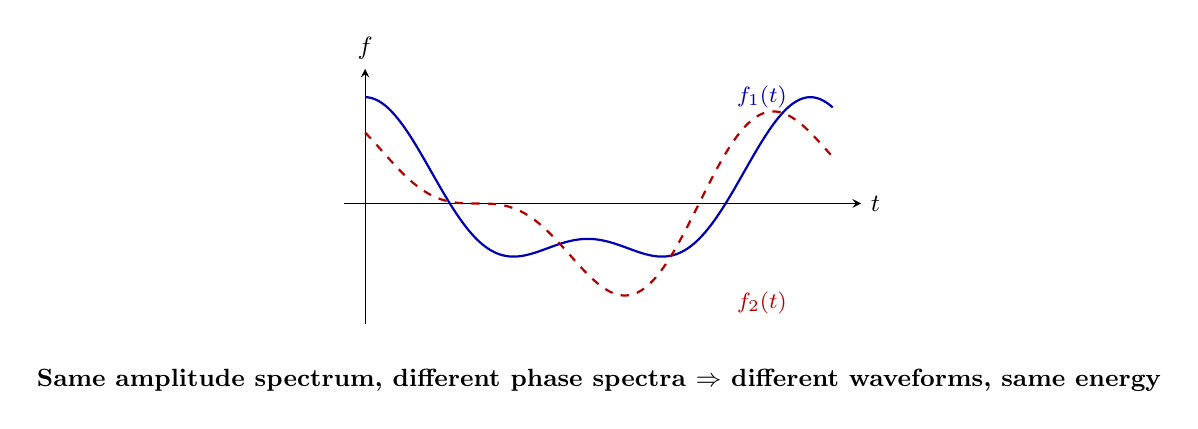
\begin{tikzpicture}[scale=0.9,>=stealth]
  \draw[->] (-0.3,0) -- (7.0,0) node[right, font=\small] {$t$};
  \draw[->] (0,-1.7) -- (0,1.9) node[above, font=\small] {$f$};

  \draw[thick, blue!70!black, domain=0:6.6, samples=200]
    plot (\x, {cos(deg(\x)) + 0.5*cos(deg(2*\x))});
  \node[blue!70!black, font=\footnotesize] at (5.6,1.5) {$f_1(t)$};

  \draw[thick, red!70!black, dashed, domain=0:6.6, samples=200]
    plot (\x, {cos(deg(\x)) - 0.5*sin(deg(2*\x))});
  \node[red!70!black, font=\footnotesize] at (5.6,-1.4) {$f_2(t)$};

  \node[font=\small\bfseries] at (3.3,-2.5) {Same amplitude spectrum, different phase spectra $\Rightarrow$ different waveforms, same energy};
\end{tikzpicture}
\caption{Comparison of two signals with the same amplitude spectrum but different phase spectra. The same amplitude spectrum guarantees the same energy (Parseval, Proposition \ref{prop:amplitude_parseval}), but the waveforms differ markedly because of the differing phases. This illustrates the irreplaceable role of phase in waveform reconstruction.}
\label{fig:same_amplitude_diff_phase}
\end{figure}

\begin{remark}[Scope and Caveats for Amplitude Series]\label{rem:amplitude_series_scope}
The amplitude series retains only the amplitudes $A_n$ and discards the phases $\phi_n$ entirely. It is therefore suited to problems independent of phase, such as energy estimation, smoothness criteria and decay-rate analysis; but it cannot be used to reconstruct the original function, to locate points of pointwise convergence, or to describe time translation or waveform symmetry. If the original series does not converge absolutely, the `amplitude series' should be understood as a formal series or a distributional series; Parseval's identity must then be used under $L^2$ or absolute-convergence conditions.
\end{remark}

\section{\texorpdfstring{Phase Series}{Phase Series}}

This section discusses the form of series with amplitude $1$ and period $2\pi$. It retains all phase information and discards amplitude information, and is the basic object for studying time translation, frequency modulation and phase coupling.

\begin{definition}[Phase Series with Amplitude $1$ and Period $2\pi$]\label{def:phase_series}
Let $\phi_n \in [0,2\pi)$ ($n \in \mathbb{Z}$) be a sequence of phases. The formal series
\[
\mathcal{P}_f(t) := \sum_{n=-\infty}^{\infty} e^{i(nt+\phi_n)}
= \sum_{n=-\infty}^{\infty} e^{i\phi_n} e^{int}
\]
is called the \textbf{phase series with amplitude $1$ and period $2\pi$}. Its generating-function form is
\[
\mathfrak{P}_f(s) := \sum_{n=-\infty}^{\infty} e^{i\phi_n} s^n.
\]
The moduli of the coefficients of a phase series are always $1$, and its information is entirely determined by the distribution of the arguments $\phi_n$. In general an infinite phase series does not converge pointwise and should be understood as a formal series, a finite truncation, or in the distributional sense.
\end{definition}

\begin{proposition}[Phase Series and Time Translation]\label{prop:phase_translation}
Let $f(t)=\sum_n A_n e^{i(nt+\phi_n)}$ have phase series $\mathcal{P}_f(t)=\sum_n e^{i(nt+\phi_n)}$. Then the phase series of the time translation $f_\tau(t):=f(t-\tau)$ is
\[
\mathcal{P}_{f_\tau}(t)
= \sum_n e^{i(nt+\phi_n-n\tau)}
= \sum_n e^{i(\phi_n-n\tau)}e^{int}.
\]
That is, a time translation is equivalent to a rotation of each term of the phase series---the rotation angle $-n\tau$ of the $n$-th term is proportional to the harmonic order $n$.
\end{proposition}

\begin{proof}
\[
f_\tau(t)=\sum_n A_n e^{i(n(t-\tau)+\phi_n)}
=\sum_n A_n e^{i(nt+\phi_n-n\tau)}.
\]
Hence the phase component is $\phi_n-n\tau$.
\end{proof}

\begin{lemma}[Bohr Mean Coefficient Formula for Phase Series]\label{lem:phase_bohr_mean}
If the phase series $\mathcal{P}_f(t)=\sum_n e^{i(nt+\phi_n)}$ converges uniformly and absolutely, then
\[
e^{i\phi_n}
= M\{\mathcal{P}_f(t)e^{-int}\}.
\]
\end{lemma}

\begin{proof}
By uniform absolute convergence,
\[
M\{\mathcal{P}_f(t)e^{-int}\}
= \sum_m e^{i\phi_m} M\{e^{i(m-n)t}\}
= e^{i\phi_n},
\]
where the last step uses Lemma \ref{lem:amplitude_exponential_mean}.
\end{proof}

\begin{theorem}[Modulus Conservation for Finite Phase Series]\label{thm:phase_modulus_conservation}
Let $S_N(t)=\sum_{n=-N}^{N} e^{i(nt+\phi_n)}$ be a finite phase series. Then
\[
\frac{1}{2\pi}\int_0^{2\pi}|S_N(t)|^2\,dt = 2N+1.
\]
That is, the total energy of a finite phase series is determined only by the number of terms and is independent of the phases $\phi_n$.
\end{theorem}

\begin{proof}
By orthogonality,
\[
|S_N(t)|^2
= \sum_{m,n=-N}^{N} e^{i((m-n)t+\phi_m-\phi_n)}.
\]
Integrating term by term:
\[
\frac{1}{2\pi}\int_0^{2\pi} e^{i(m-n)t}\,dt = \delta_{mn}.
\]
Hence only the diagonal terms $m=n$ survive, each contributing $1$, giving $2N+1$ in total.
\end{proof}

\begin{corollary}[Phase Rotation Rule for Time Translation]\label{cor:phase_time_shift_rotation}
A time translation $t\mapsto t-\tau$ multiplies the $n$-th term of the phase series by $e^{-in\tau}$. Therefore:
\begin{enumerate}[label=(\roman*)]
    \item if $\tau=2\pi k$, all terms are unchanged;
    \item if $\tau=\pi$, the $n$-th term is multiplied by $(-1)^n$;
    \item if $\tau$ is an irrational multiple of $2\pi$, the phase rotation no longer has periodicity of finite order.
\end{enumerate}
\end{corollary}

\begin{proof}
By Proposition \ref{prop:phase_translation}, the phase of the $n$-th term becomes $\phi_n-n\tau$. Substituting in each case gives the result.
\end{proof}

\begin{property}[Basic Properties of Phase Series]\label{prop:phase_series_properties}
\begin{enumerate}[label=(\roman*)]
    \item \textbf{Unit-modulus coefficients}: all coefficients satisfy $|e^{i\phi_n}|=1$;
    \item \textbf{Conjugate symmetry}: a real signal requires $e^{i\phi_{-n}}=e^{-i\phi_n}$, that is $\phi_{-n}=-\phi_n \pmod{2\pi}$;
    \item \textbf{Translation as rotation}: a time translation is equivalent to term-by-term phase rotation;
    \item \textbf{Conservation of energy in the number of terms}: the total energy of a finite truncation equals the number of terms;
    \item \textbf{The fully infinite series generally does not converge}: $\sum_{n\in\mathbb{Z}}e^{int}$ does not converge pointwise and should be understood in the distributional sense.
\end{enumerate}
\end{property}

\begin{proof}
(i) By definition. (ii) A real signal requires $c_{-n}=\overline{c_n}$; here $c_n=e^{i\phi_n}$, so $e^{i\phi_{-n}}=e^{-i\phi_n}$. (iii) By Proposition \ref{prop:phase_translation}. (iv) By Theorem \ref{thm:phase_modulus_conservation}. (v) The general term has modulus $1$ and does not tend to zero, so the series diverges in the usual sense; as a distribution, $\sum_{n\in\mathbb{Z}}e^{int}=2\pi\sum_{k\in\mathbb{Z}}\delta(t-2\pi k)$.
\end{proof}

\begin{example}[Linear Phase and Time Translation]\label{ex:linear_phase}
Take $\phi_n=-n\tau$. Then
\[
\mathcal{P}(t)=\sum_{n=-N}^{N} e^{i(nt-n\tau)}
= \sum_{n=-N}^{N} e^{in(t-\tau)}
= D_N(t-\tau),
\]
where $D_N$ is the Dirichlet kernel. This example shows that a linear phase corresponds to a time translation.
\end{example}

\begin{proposition}[The rotation--translation duality of the phase series]\label{prop:phase_rotation_translation_duality}
Let the phase series be $\mathcal{P}_f(t) = \sum_n e^{i(nt+\phi_n)}$. Then:
\begin{enumerate}[label=(\roman*)]
  \item \textbf{Time translation} $t \mapsto t - \tau$ is equivalent to multiplying the $n$-th term by $e^{-in\tau}$ in the frequency domain (Proposition \ref{prop:phase_translation});
  \item \textbf{Frequency translation} $n \mapsto n + k$ is equivalent to multiplying the $n$-th term by $e^{ikt}$ in the time domain.
\end{enumerate}
This is the manifestation on phase series of the \textbf{translation--modulation duality} of the Fourier transform.
\end{proposition}

\begin{proof}
(i) Given directly by Proposition \ref{prop:phase_translation}. (ii) The frequency translation $n \mapsto n + k$ turns the $n$-th term $e^{i(nt+\phi_n)}$ into $e^{i((n+k)t+\phi_{n+k})}$, that is, it multiplies the original $(n+k)$-th term by $e^{ikt}$.
\end{proof}

\begin{example}[Linear phase and group delay]\label{ex:linear_phase_group_delay}
Let $\phi_n = -n\tau$ (linear phase). Then the group delay of the phase series is
\[
\tau_g(n) = -\frac{d\phi_n}{dn} = \tau,
\]
that is, all frequency components have the same group delay. In signal processing a system with constant group delay is called a \textbf{linear phase system}, corresponding to a pure translation $t \mapsto t - \tau$ in the time domain (Example \ref{ex:linear_phase}).
\end{example}

\begin{property}[Parseval's identity for the phase series (finitely many terms)]\label{prop:phase_parseval_finite}
Let $\mathcal{P}_N(t) = \sum_{n=-N}^{N} A_n e^{i(nt+\phi_n)}$ be a finite phase series ($A_n > 0$, not necessarily equal to $1$). Then
\[
\frac{1}{2\pi}\int_0^{2\pi} |\mathcal{P}_N(t)|^2\,dt = \sum_{n=-N}^{N} A_n^2.
\]
\end{property}

\begin{proof}
By the orthogonality of the Fourier basis (Proposition \ref{prop:fourier_orthogonality}), the cross terms integrate to zero and only the diagonal terms remain.
\end{proof}

\begin{figure}[htbp]
\centering
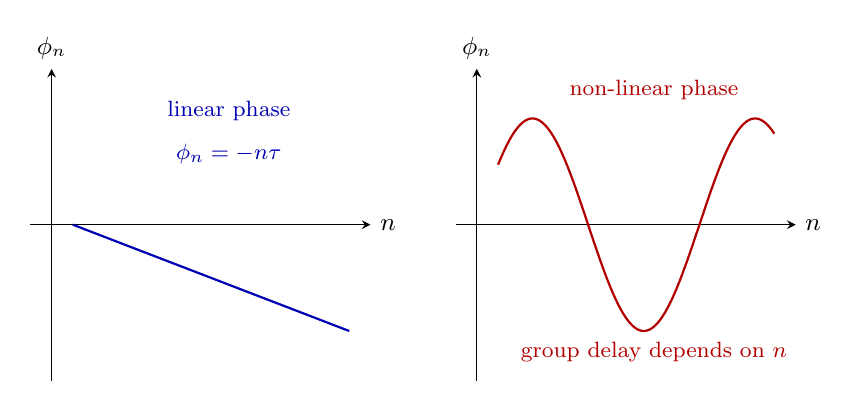
\begin{tikzpicture}[scale=0.9,>=stealth]
  \begin{scope}
    \draw[->] (-0.3,0) -- (4.5,0) node[right, font=\small] {$n$};
    \draw[->] (0,-2.2) -- (0,2.2) node[above, font=\small] {$\phi_n$};

    \draw[thick, blue!70!black] (0.3,0) -- (4.2,-1.5);
    \node[blue!70!black, font=\footnotesize] at (2.5,1.6) {linear phase};
    \node[blue!70!black, font=\footnotesize] at (2.5,1.0) {$\phi_n = -n\tau$};
  \end{scope}

  \begin{scope}[xshift=6.0cm]
    \draw[->] (-0.3,0) -- (4.5,0) node[right, font=\small] {$n$};
    \draw[->] (0,-2.2) -- (0,2.2) node[above, font=\small] {$\phi_n$};

    \draw[thick, red!70!black, domain=0.3:4.2, samples=100]
      plot (\x, {1.5*sin(deg(2*\x))});
    \node[red!70!black, font=\footnotesize] at (2.5,1.9) {non-linear phase};
    \node[red!70!black, font=\footnotesize] at (2.5,-1.8) {group delay depends on $n$};
  \end{scope}
\end{tikzpicture}
\caption{Two typical shapes of a phase spectrum. Left: linear phase (constant group delay), corresponding to a pure translation in the time domain. Right: non-linear phase (group delay depending on frequency), corresponding to waveform distortion in the time domain.}
\label{fig:phase_spectrum_examples}
\end{figure}

\begin{remark}[Scope and Caveats for Phase Series]\label{rem:phase_series_scope}
The phase series retains only the phases $e^{i\phi_n}$ and discards the amplitudes $A_n$ entirely. It is therefore suited to problems such as time translation, phase coupling, frequency modulation and synchronisation analysis; but it cannot by itself give the energy distribution, the rate of convergence or the magnitude of function values. A fully infinite phase series generally does not converge and must be used together with finite truncation, window functions or distribution theory. The product term $-n\tau$ of phase and frequency shows that the `rotation' in a phase series is tied to the harmonic order $n$; this is a basic manifestation of the frequency--phase duality.
\end{remark}

\section{\texorpdfstring{Frequency Series and the Hierarchy of Series}{Frequency Series and the Hierarchy of Series}}

After the amplitude series and the phase series, this section establishes the \textbf{frequency series} and gives the five levels of the hierarchy of series. The frequency series retains only the frequency-lattice structure and discards amplitude and phase information entirely.

\begin{definition}[Frequency Series]\label{def:frequency_series}
Let $f$ have period $T$, with Fourier expansion
\[
f(t)=\sum_{n} A_n e^{i(\omega_n t+\phi_n)}, \qquad \omega_n=\frac{2\pi n}{T}.
\]
The \textbf{frequency series} of $f$ is defined as the formal series that retains only the frequency components
\[
\mathcal{F}_f(s) := \sum_{n=-\infty}^{\infty} \omega_n s^n
= \frac{2\pi}{T}\sum_{n=-\infty}^{\infty} n s^n.
\]
The frequency series discards all amplitude and phase information and retains only the frequency lattice of each harmonic. The frequency series is entirely determined by the fundamental period $T$---all frequencies are integer multiples of the fundamental frequency $\omega_0=2\pi/T$. Scaling property of the frequency series: a change of period to $\lambda T$ ($\lambda>0$) sends $\omega_n\mapsto \omega_n/\lambda$, that is, it scales the frequency series as a whole by $1/\lambda$.
\end{definition}

\begin{proposition}[Frequency Series and Period Scaling]\label{prop:frequency_scaling}
Let $f$ have period $T$, with frequency series
\[
\mathcal{F}_f(s)=\frac{2\pi}{T}\sum_n n s^n.
\]
Then the frequency series of the time scaling $f_\lambda(t):=f(t/\lambda)$ ($\lambda>0$) is
\[
\mathcal{F}_{f_\lambda}(s)
= \frac{2\pi}{\lambda T}\sum_n n s^n
= \frac{1}{\lambda}\mathcal{F}_f(s).
\]
That is, scaling time by a factor $\lambda$ is equivalent to scaling the frequency series as a whole by $1/\lambda$---this is the manifestation of the frequency--period duality at the level of series.
\end{proposition}

\begin{proof}
$f_\lambda(t)=f(t/\lambda)$ has period $\lambda T$, so its Fourier frequencies are
\[
\omega_n^{(\lambda)}=\frac{2\pi n}{\lambda T}=\frac{\omega_n}{\lambda}.
\]
Hence the frequency series is scaled as a whole by $1/\lambda$.
\end{proof}

\begin{definition}[The Five-Level Hierarchy of Series]\label{def:series_five_layers}
For a function $f$ of period $T$, its series decompositions are arranged in increasing order of information content as:
\begin{enumerate}[label=(\roman*)]
    \item \textbf{Frequency series} $\mathcal{F}_f$: retains only the frequency lattice $\omega_n=2\pi n/T$, and is entirely determined by the fundamental period $T$.
    \item \textbf{Amplitude series} $\mathcal{A}_f$: retains the amplitudes $A_n$ and discards the phases $\phi_n$ and the frequency-lattice structure.
    \item \textbf{Phase series} $\mathcal{P}_f$: retains the phases $e^{i\phi_n}$ and discards the amplitudes $A_n$ and the frequency-lattice structure.
    \item \textbf{Fourier series}: retains the amplitudes $A_n$ and the phases $\phi_n$, with the frequency lattice fixed by $T$.
    \item \textbf{Periodic series}: retains the four-tuple of amplitudes $A_{p,n}$, frequencies $\omega_{p,n}$, phases $\phi_{p,n}$ and periods $T_p$, and is the complete decomposition into multiple period layers.
\end{enumerate}
The relation among the five levels is: Fourier series $=$ amplitude series $\times$ phase series (term by term); periodic series $=$ the sum of the Fourier series of the multiple period layers; the amplitude series, the phase series and the frequency series are respectively the projections of the Fourier series onto its amplitude, phase and frequency components.
\end{definition}

\begin{proposition}[Reconstruction Relations among the Five Levels]\label{prop:series_five_layers_reconstruction}
With the above notation:
\begin{enumerate}[label=(\roman*)]
    \item From the amplitude series and the phase series the Fourier coefficients can be reconstructed: $c_n=A_n e^{i\phi_n}$, and hence the Fourier series.
    \item From the amplitude series the energy can be reconstructed: $\frac{1}{T}\int_0^T |f|^2=\sum_n A_n^2$ (Parseval).
    \item From the phase series the effect of time translation can be reconstructed: $\phi_n-2\pi n\tau/T$.
    \item From the frequency series the effect of period scaling can be reconstructed: $\omega_n\mapsto \omega_n/\lambda$.
    \item The information of any single one of the five levels is insufficient to reconstruct $f$; only when the four-tuple is complete (the periodic series) can $f$ be reconstructed in full.
\end{enumerate}
\end{proposition}

\begin{proof}
(i) Given directly by $c_n=A_n e^{i\phi_n}$.
(ii) By Proposition \ref{prop:amplitude_parseval}.
(iii) By Proposition \ref{prop:phase_translation}.
(iv) By Proposition \ref{prop:frequency_scaling}.
(v) It follows from the term-by-term comparison of information in Definition \ref{def:series_five_layers}: the frequency series contains only $\omega_n$, the amplitude series only $A_n$, and the phase series only $e^{i\phi_n}$; any one of them lacks the information of the other components.
\end{proof}

\begin{example}[An explicit comparison of the five series levels]\label{ex:five_layers_example}
Take the periodic function $f(t) = 3 + 2 e^{i(t + \pi/3)} + e^{i(3t - \pi/4)}$ of period $T = 2\pi$. The series at the five levels are respectively:
\begin{center}
\begin{tabular}{@{}p{2.8cm}p{9.0cm}@{}}
\toprule
Level & Explicit form \\
\midrule
Frequency series & $\mathcal{F}_f(s) = \sum_n n s^n$, retaining only the frequency lattice $\{0, 1, 3\}$ (modulo $2\pi$) \\
Amplitude series & $\mathcal{A}_f(t) = 3 + 2 e^{it} + e^{i3t}$, amplitudes $\{3, 2, 1\}$ \\
Phase series & $\mathcal{P}_f(t) = e^{i\pi/3} e^{it} + e^{-i\pi/4} e^{i3t}$, phases $\{\pi/3, -\pi/4\}$ \\
Fourier series & $f(t) = 3 + 2 e^{i(t+\pi/3)} + e^{i(3t-\pi/4)}$ \\
Periodic series & the Fourier series on the single period layer $P = \{2\pi\}$ \\
\bottomrule
\end{tabular}
\end{center}
This example shows that, among the five levels, only the Fourier series and the periodic series (which coincide in the single-period-layer case) can reconstruct $f$ in full; the frequency series, the amplitude series and the phase series each retain only one component.
\end{example}

\begin{figure}[htbp]
\centering
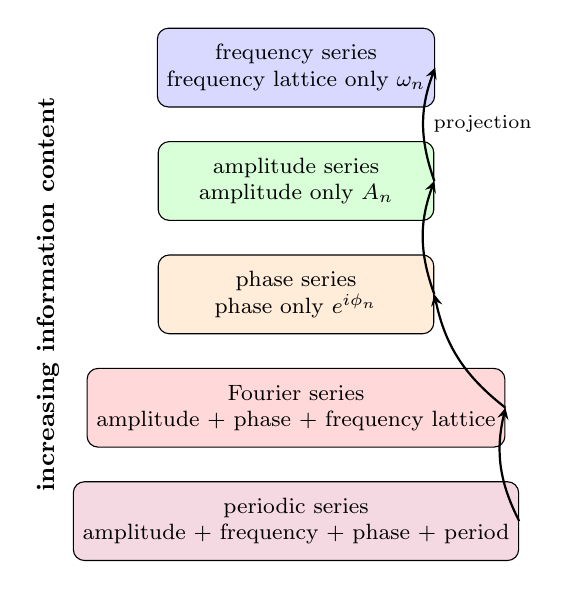
\begin{tikzpicture}[scale=0.9,>=stealth,
  layer/.style={draw, rounded corners, minimum width=3.5cm, minimum height=1.0cm, align=center, font=\footnotesize},
  arrow/.style={->, thick, >=stealth}]

  \node[layer, fill=blue!15] (freq) at (0,0) {frequency series\\frequency lattice only $\omega_n$};
  \node[layer, fill=green!15] (amp) at (0,-1.6) {amplitude series\\amplitude only $A_n$};
  \node[layer, fill=orange!15] (phase) at (0,-3.2) {phase series\\phase only $e^{i\phi_n}$};
  \node[layer, fill=red!15] (fourier) at (0,-4.8) {Fourier series\\amplitude $+$ phase $+$ frequency lattice};
  \node[layer, fill=purple!15] (periodic) at (0,-6.4) {periodic series\\amplitude $+$ frequency $+$ phase $+$ period};

  \draw[arrow] (amp.east) to[bend left=20] node[right, font=\scriptsize, align=left] {projection} (freq.east);
  \draw[arrow] (phase.east) to[bend left=20] (amp.east);
  \draw[arrow] (fourier.east) to[bend left=20] (phase.east);
  \draw[arrow] (periodic.east) to[bend left=20] (fourier.east);

  \node[font=\small\bfseries, rotate=90] at (-3.5,-3.2) {increasing information content};

\end{tikzpicture}
\caption{The five levels of the hierarchy of series. The information content increases level by level from the frequency series (frequency lattice only) to the periodic series (complete four-tuple); each level is a projection or a synthesis of the level above.}
\label{fig:series_five_layers}
\end{figure}

\section{\texorpdfstring{Periodic Series: Complete Decomposition via Four-Tuples}{Periodic Series}}

\begin{definition}[Periodic Series (Complex Form)]\label{def:periodic_series}
Let $P$ be a finite or countable \textbf{set of period-class indices}, let a fundamental period $T_p > 0$ be assigned to each $p \in P$, and let $n \in \mathbb{Z}$ be the harmonic order within that period class. A series of the form
\[
f(t) = \sum_{p \in P} \sum_{n \in \mathbb{Z}} A_{p,n}\, e^{i(2\pi n t / T_p + \phi_{p,n})}
\]
is called a \textbf{periodic series} (complex form), in which the $(p,n)$-th term is determined by the \textbf{four-tuple} $(A_{p,n}, \omega_{p,n}, \phi_{p,n}, T_p)$:
\begin{enumerate}[label=(\roman*)]
    \item $A_{p,n} \ge 0$ is called the \textbf{amplitude component};
    \item $\omega_{p,n} := 2\pi n / T_p$ is called the \textbf{frequency component};
    \item $\phi_{p,n} \in [0, 2\pi)$ is called the \textbf{phase component};
    \item $T_p$ is called the \textbf{period component} (the primary index).
\end{enumerate}
Frequency and period are tied by the \textbf{fixed-length relation} $\omega_{p,n} = 2\pi n / T_p$. Writing the polar-form coefficients $c_{p,n} = A_{p,n} e^{i\phi_{p,n}}$, we have $f(t) = \sum_{p,n} c_{p,n} e^{i\omega_{p,n} t}$.
\end{definition}

\begin{definition}[Periodic Series (Real Form)]\label{def:periodic_series_real}
Let $f: \mathbb{R} \to \mathbb{R}$. A series of the form
\[
f(t) = \sum_{p \in P} \sum_{n \in \mathbb{Z}} A_{p,n} \cos\!\big( \tfrac{2\pi n}{T_p} t + \phi_{p,n} \big), \qquad A_{p,n} \ge 0,\ \phi_{p,n} \in [0, 2\pi)
\]
is called a \textbf{periodic series} (real form).
\end{definition}

\begin{proposition}[Equivalence of Real and Complex Forms]\label{prop:periodic_series_real_complex}
The real-form periodic series is the real part of the complex-form periodic series.
\end{proposition}

\begin{proof}
It follows directly from Euler's formula $e^{i\theta} = \cos\theta + i\sin\theta$.
\end{proof}

\begin{proposition}[Fourier Series as a Special Case of Periodic Series]\label{prop:fourier_as_periodic_series}
The Fourier series is the special case of the periodic series on a single period layer ($P = \{T\}$).
\end{proposition}

\begin{proof}
For a $T$-periodic function the Bohr mean reduces to a single-period average:
\[
M\{g\} = \frac{1}{T}\int_0^T g(t)\,dt.
\]
Hence the periodic series degenerates to the Fourier series.
\end{proof}

\begin{proposition}[Periodic Series as a Synthesis of Amplitude, Phase, and Frequency Series]\label{prop:periodic_series_synthesis}
Let the periodic series be
\[
f(t)=\sum_{p\in P}\sum_{n\in\mathbb Z}A_{p,n}e^{i(\omega_{p,n}t+\phi_{p,n})},
\qquad \omega_{p,n}=\frac{2\pi n}{T_p}.
\]
For each period layer $p\in P$, write
\[
\mathcal A_p(s)=\sum_n A_{p,n}s^n,\qquad
\mathcal P_p(s)=\sum_n e^{i\phi_{p,n}}s^n,\qquad
\mathcal F_p(s)=\sum_n \omega_{p,n}s^n.
\]
Then:
\begin{enumerate}[label=(\roman*)]
    \item if the single period layer $P=\{T\}$, $T=2\pi$ is fixed and all $\phi_{p,n}=0$ are set, then $f$ degenerates to the amplitude series
    \[
    \sum_n A_n e^{int};
    \]
    \item if the single period layer $P=\{T\}$, $T=2\pi$ is fixed and all $A_{p,n}=1$ are set, then $f$ degenerates to the phase series
    \[
    \sum_n e^{i(nt+\phi_n)};
    \]
    \item if the single period layer is fixed and only the frequency parameters $\omega_n=2\pi n/T$ are retained, the frequency series is obtained;
    \item in general the periodic series is formed by synthesising the four-tuple of amplitude $A_{p,n}$, phase $\phi_{p,n}$, frequency $\omega_{p,n}$ and period $T_p$ according to the period layer $p$.
\end{enumerate}
\end{proposition}

\begin{proof}
(i)(ii)(iii) Follow directly from Definitions \ref{def:periodic_series}, \ref{def:amplitude_series}, \ref{def:phase_series}, \ref{def:frequency_series} by taking the corresponding parameters. (iv) From
\[
c_{p,n}=A_{p,n}e^{i\phi_{p,n}},\qquad \omega_{p,n}=\frac{2\pi n}{T_p}
\]
it is read off directly.
\end{proof}

\begin{corollary}[The Three Series as Projections of the Periodic Series]\label{cor:periodic_series_projections}
The amplitude series, the phase series and the frequency series are respectively the projections of the periodic series onto its amplitude, phase and frequency components. Any single projection is insufficient to reconstruct $f$; when the four-tuple is complete, $f$ can be reconstructed uniquely.
\end{corollary}

\begin{proof}
By Proposition \ref{prop:periodic_series_synthesis} and Proposition \ref{prop:series_five_layers_reconstruction}.
\end{proof}

\begin{remark}[The Precise Meaning of `Synthesis']\label{rem:periodic_series_synthesis_scope}
`The periodic series is a synthesis of the three series' should be understood as follows: taking the period $T_p$ as the primary index, within each period layer the amplitude series provides $A_{p,n}$, the phase series provides $e^{i\phi_{p,n}}$ and the frequency series provides $\omega_{p,n}=2\pi n/T_p$, and then, through
\[
A_{p,n}e^{i(\omega_{p,n}t+\phi_{p,n})}
\]
they are combined into a periodic series. It is not the term-by-term sum of the three formal series, but a layered Fourier synthesis parametrised by the four-tuple. When the single period layer is $P=\{T\}$, $T=2\pi$ it degenerates to the Fourier series; taking the phase to be zero or the amplitude to be one then gives the amplitude series or the phase series respectively.
\end{remark}

\begin{example}[Quasi-Periodic Periodic Series]\label{ex:quasi_periodic_series}
\[
f(t) = 3 e^{i(\sqrt{2}\,t + \pi/6)} + 2 e^{i(t - \pi/3)}.
\]
The frequencies $\sqrt{2}$ and $1$ are incommensurable, so $f$ is a quasi-periodic function.
\end{example}

\begin{property}[Degeneration of the periodic series to a Fourier series]\label{prop:periodic_series_degeneration}
When the set of period-class indices $P = \{T\}$ is a singleton, the periodic series degenerates to the Fourier series of period $T$:
\[
f(t) = \sum_{n \in \mathbb{Z}} A_n e^{i(2\pi n t / T + \phi_n)}.
\]
Furthermore, if $T = 2\pi$, it degenerates to the standard Fourier series $f(t) = \sum_{n \in \mathbb{Z}} c_n e^{int}$.
\end{property}

\begin{proof}
For the single period layer $P = \{T\}$ the outer sum disappears and the inner sum is precisely the Fourier series form. Taking $T = 2\pi$ gives the standard form.
\end{proof}

\begin{example}[A periodic series with two period layers]\label{ex:two_period_layers}
Take $P = \{2\pi, 2\pi\sqrt{2}\}$ and construct
\[
f(t) = 3 e^{i(t + \pi/6)} + 2 e^{i(\sqrt{2}\,t - \pi/3)}.
\]
This function has \textbf{two independent period layers}: the outer one is the component of period $2\pi$ and the inner one the component of period $2\pi\sqrt{2}$. Since $2\pi/(2\pi\sqrt{2}) = 1/\sqrt{2} \notin \mathbb{Q}$, the two layers are incommensurable and $f$ is a quasi-periodic function (Example \ref{ex:quasi_periodic_series}).
\end{example}

\begin{theorem}[A sufficient condition for convergence of the periodic series]\label{thm:periodic_series_convergence}
Let the periodic series $f(t) = \sum_{p \in P} \sum_{n \in \mathbb{Z}} A_{p,n} e^{i(\omega_{p,n} t + \phi_{p,n})}$ satisfy
\[
\sum_{p \in P} \sum_{n \in \mathbb{Z}} A_{p,n} < \infty.
\]
Then $f$ converges uniformly and absolutely on $\mathbb{R}$, and $f$ is continuous and bounded.
\end{theorem}

\begin{proof}
For any $t$, $|A_{p,n} e^{i(\omega_{p,n} t + \phi_{p,n})}| = A_{p,n}$. By the Weierstrass M-test (Theorem \ref{thm:weierstrass_mtest}) the series converges uniformly. Continuity and boundedness are preserved by uniform convergence.
\end{proof}

\subsection{\texorpdfstring{The Unit-Coefficient Special Case: Zero Phase and Unit Amplitude}{The Unit-Coefficient Special Case: Zero Phase and Unit Amplitude}}

This subsection discusses the special form of the periodic series when the phase is zero and the amplitude is one. It is the normalised-basis special case of the general Fourier series and also the entry point for understanding orthogonal expansions and distributional convergence.

\begin{definition}[Periodic Series with Zero Phase and Unit Amplitude]\label{def:unit_phase_zero_amplitude_series}
Let $S \subseteq \mathbb{Z}$ be a set of frequency indices and $T>0$. The formal series
\[
\Phi_{T,S}(t) := \sum_{n \in S} e^{i 2\pi n t/T}
\]
is called the \textbf{periodic series with zero phase and unit amplitude}. When $T=2\pi$ we abbreviate it as
\[
\Phi_S(t) := \sum_{n \in S} e^{i n t}.
\]
Its real form (requiring $S=-S$) is
\[
\Phi_S^{\mathbb{R}}(t) := \sum_{n \in S} \cos(nt).
\]
If $S$ is a finite set, then $\Phi_{T,S}$ is a trigonometric polynomial converging absolutely pointwise; if $S=\mathbb{Z}$, it should be understood in the distributional sense.
\end{definition}

\begin{proposition}[Normalisation of Coefficients, Phase, and Amplitude]\label{prop:unit_phase_zero_coefficients}
The Fourier coefficients of the periodic series with zero phase and unit amplitude $\Phi_{T,S}(t)=\sum_{n\in S}e^{i2\pi n t/T}$ are
\[
c_n =
\begin{cases}
1, & n\in S,\\
0, & n\notin S.
\end{cases}
\]
Hence its amplitudes are $A_n=1$ ($n\in S$) and its phases are $\phi_n=0$ ($n\in S$).
\end{proposition}

\begin{proof}
By the Fourier coefficient formula and orthogonality (Proposition \ref{prop:fourier_orthogonality}),
\[
c_n=\frac{1}{T}\int_0^T \Phi_{T,S}(t)e^{-i2\pi n t/T}\,dt
=\sum_{m\in S}\frac{1}{T}\int_0^T e^{i2\pi (m-n)t/T}\,dt
=\sum_{m\in S}\delta_{mn}.
\]
Hence $c_n=1$ when $n\in S$ and $c_n=0$ otherwise.
\end{proof}

\begin{lemma}[$L^2$ Orthogonality of a Finite Frequency Set]\label{lem:unit_phase_zero_orthogonality}
Let $S\subset \mathbb{Z}$ be finite. Then
\[
\frac{1}{T}\int_0^T \Phi_{T,S}(t)\overline{\Phi_{T,S}(t)}\,dt = |S|,
\]
where $|S|$ is the number of elements of $S$. More generally,
\[
\frac{1}{T}\int_0^T e^{i2\pi m t/T}e^{-i2\pi n t/T}\,dt=\delta_{mn}.
\]
\end{lemma}

\begin{proof}
Expanding:
\[
\frac{1}{T}\int_0^T \Phi_{T,S}\overline{\Phi_{T,S}}\,dt
=\sum_{m,n\in S}\frac{1}{T}\int_0^T e^{i2\pi (m-n)t/T}\,dt
=\sum_{m,n\in S}\delta_{mn}=|S|.
\]
\end{proof}

\begin{theorem}[Relation between the Zero-Phase, Unit-Amplitude Periodic Series and General Fourier Series]\label{thm:unit_phase_zero_fourier_relation}
Let $f$ have period $T$, with Fourier series
\[
f(t)\sim \sum_{n\in\mathbb{Z}} c_n e^{i2\pi n t/T},
\qquad c_n=A_n e^{i\phi_n}.
\]
Then:
\begin{enumerate}[label=(\roman*)]
    \item the general Fourier series is the term-by-term product of the amplitude series and the phase series:
    \[
    c_n e^{i2\pi n t/T}
    = A_n e^{i\phi_n}e^{i2\pi n t/T}.
    \]
    \item the periodic series with zero phase and unit amplitude is the normalised special case of the Fourier series when $c_n=1$ ($n\in S$):
    \[
    \Phi_{T,S}(t)=\sum_{n\in S}1\cdot e^{i\phi_n}e^{i2\pi n t/T},
    \qquad \phi_n=0,\ A_n=1.
    \]
    \item if $S$ is finite, then $\Phi_{T,S}$ is the orthogonal projection kernel on $L^2([0,T])$ spanned by the frequency set $S$; if $S=\mathbb{Z}$, then $\Phi_{T,\mathbb{Z}}$ is the distributional limit of the periodic Dirichlet kernel:
    \[
    \sum_{n\in\mathbb{Z}}e^{i2\pi n t/T}
    = T\sum_{k\in\mathbb{Z}}\delta(t-kT).
    \]
\end{enumerate}
\end{theorem}

\begin{proof}
(i) Write it out directly from $c_n=A_n e^{i\phi_n}$.
(ii) Take $A_n=1$, $\phi_n=0$ ($n\in S$) and $c_n=0$ otherwise in (i).
(iii) For finite $S$, $\Phi_{T,S}$ is the sum of finitely many orthogonal basis functions, and its integral-kernel property is given by Lemma \ref{lem:unit_phase_zero_orthogonality}. For $S=\mathbb{Z}$, use the Poisson summation formula (or the limit of the Dirichlet kernel in the distributional sense):
\[
\sum_{n\in\mathbb{Z}}e^{i2\pi n t/T}
= T\sum_{k\in\mathbb{Z}}\delta(t-kT).
\]
Hence it should be understood distributionally.
\end{proof}

\begin{corollary}[Parseval's Identity for Finite Normalised Bases]\label{cor:unit_phase_zero_parseval}
Let $S\subset\mathbb{Z}$ be finite. Then
\[
\frac{1}{T}\int_0^T |\Phi_{T,S}(t)|^2\,dt = |S|.
\]
That is, the energy of a finite periodic series with zero phase and unit amplitude equals the number of frequency terms.
\end{corollary}

\begin{proof}
Obtained directly from Lemma \ref{lem:unit_phase_zero_orthogonality}.
\end{proof}

\begin{property}[Basic Properties of the Zero-Phase, Unit-Amplitude Periodic Series]\label{prop:unit_phase_zero_properties}
\begin{enumerate}[label=(\roman*)]
    \item \textbf{Unit coefficients}: on $S$, $c_n=1$, the amplitude is $1$ and the phase is $0$;
    \item \textbf{Orthogonality}: terms of different frequencies are orthogonal in $L^2$;
    \item \textbf{Additivity of finite energy}: the energy of a finite truncation equals the number of terms;
    \item \textbf{The real form is a sum of cosines}: if $S=-S$, the real form is $\sum_{n\in S}\cos(2\pi n t/T)$;
    \item \textbf{Distributional nature at all frequencies}: when $S=\mathbb{Z}$ the series does not converge pointwise, but is a periodic $\delta$ comb.
\end{enumerate}
\end{property}

\begin{proof}
(i) By Proposition \ref{prop:unit_phase_zero_coefficients}. (ii) By Lemma \ref{lem:unit_phase_zero_orthogonality}. (iii) By Corollary \ref{cor:unit_phase_zero_parseval}. (iv) By Euler's formula. (v) By Theorem \ref{thm:unit_phase_zero_fourier_relation}(iii).
\end{proof}

\begin{example}[Dirichlet Kernel as a Finite Normalised Periodic Series]\label{ex:dirichlet_kernel_truncation}
Taking $T=2\pi$ and $S=\{-N,\dots,N\}$ gives
\[
\Phi_{\{-N,\dots,N\}}(t)
=\sum_{n=-N}^{N}e^{int}
=D_N(t)
=\frac{\sin((N+\tfrac12)t)}{\sin(t/2)}.
\]
Its energy is
\[
\frac{1}{2\pi}\int_0^{2\pi}|D_N(t)|^2\,dt=2N+1.
\]
As $N\to\infty$, $D_N$ tends in the distributional sense to $2\pi\sum_{k\in\mathbb{Z}}\delta(t-2\pi k)$.
\end{example}

\begin{remark}[Scope of the Zero-Phase, Unit-Amplitude Periodic Series]\label{rem:unit_phase_zero_scope}
The zero-phase, unit-amplitude periodic series is the `unit coefficient' special case of the Fourier series, suited to illustrating orthogonal bases, the Dirichlet kernel, Poisson summation and distributional convergence. It does not represent a general $L^2$ or continuous periodic function, because the unit-coefficient series over all frequencies does not converge; it has a rigorous meaning only for a finite frequency set or in the distributional sense. For real signals one must further require the frequency set to be symmetric about the origin and take the real part. Its relation to the general Fourier series is: general series $=$ amplitude series $\times$ phase series, whilst the case of this subsection is the normalised intersection in which all amplitudes are $1$ and all phases are $0$.
\end{remark}

\subsection{\texorpdfstring{Bohr Means and the Determination of Coefficients}{Bohr Means and the Determination of Coefficients}}

\begin{definition}[Bohr Mean]\label{def:bohr_mean}
Let $f: \mathbb{R} \to \mathbb{C}$. If the limit
\[
M\{f\} := \lim_{T \to \infty} \frac{1}{2T} \int_{-T}^{T} f(t)\,dt
\]
exists, it is called the \textbf{Bohr mean} of $f$.
\end{definition}

\begin{lemma}[Bohr Mean of Exponential Functions]\label{lem:bohr_mean_exponential}
For any $\omega \in \mathbb{R}$,
\[
M\{e^{i\omega t}\} =
\begin{cases}
1, & \omega = 0, \\
0, & \omega \neq 0.
\end{cases}
\]
\end{lemma}

\begin{proof}
When $\omega = 0$ the integrand is identically $1$. When $\omega \neq 0$,
\[
\frac{1}{2T}\int_{-T}^{T} e^{i\omega t}\,dt = \frac{\sin(\omega T)}{\omega T} \to 0 \qquad (T \to \infty).
\]
\end{proof}

\begin{proposition}[Elementary Proof in the Finite Case: Vandermonde Determinant]\label{prop:vandermonde_uniqueness}
Let the frequencies $\omega_1 < \cdots < \omega_N$ be pairwise distinct. If $\sum_{k=1}^{N} c_k e^{i\omega_k t} \equiv 0$, then $c_1 = \cdots = c_N = 0$.
\end{proposition}

\begin{proof}
Differentiating the identity successively $j = 0, \dots, N-1$ times and evaluating at $t = 0$ gives a homogeneous linear system whose coefficient matrix is a Vandermonde matrix with non-zero determinant.
\end{proof}

\begin{theorem}[Determination of Periodic-Series Coefficients (Bohr)]\label{thm:periodic_series_bohr}
Let the periodic series $f(t) = \sum_{p,n} A_{p,n} e^{i(\omega_{p,n} t + \phi_{p,n})}$ converge uniformly on $\mathbb{R}$, with all frequencies pairwise distinct. Then
\[
A_{p,n} e^{i\phi_{p,n}} = M\big\{ f(t)\, e^{-i\omega_{p,n} t} \big\}.
\]
\end{theorem}

\begin{proof}
By uniform convergence the integral and the sum may be interchanged. By Lemma \ref{lem:bohr_mean_exponential} the cross terms have zero mean and only the $(p,n)$ term survives.
\end{proof}

\begin{corollary}[Uniqueness of Representation]\label{cor:periodic_series_unique}
If two uniformly convergent periodic series are equal as functions and have the same period partition $P$ and the same frequency set, then their amplitudes and phases agree term by term.
\end{corollary}

\begin{proof}
It follows directly from Theorem \ref{thm:periodic_series_bohr}.
\end{proof}

\begin{theorem}[Generalised Parseval Identity (Bohr)]\label{thm:bohr_parseval}
Let the periodic series $f(t) = \sum_{p,n} c_{p,n} e^{i\omega_{p,n} t}$ satisfy $\sum_{p,n} |c_{p,n}| < \infty$. Then
\[
M\{|f|^2\} = \sum_{p,n} |c_{p,n}|^2 = \sum_{p,n} A_{p,n}^2.
\]
\end{theorem}

\begin{proof}
Expand $|f(t)|^2$; by absolute convergence the Bohr mean may be interchanged with the summation, the cross terms have zero mean, and the diagonal terms give $|c_{p,n}|^2$.
\end{proof}

\subsection{\texorpdfstring{The Periodic Transform: Unification of the Classical Integral Transforms}{The Periodic Transform}}

\begin{definition}[Periodic Transform (Frequency-Dictionary Form)]\label{def:periodic_transform}
Let $\Lambda = \{\omega_k\}_{k \in K}$ be a \textbf{frequency dictionary}. For a function $f$, its \textbf{periodic transform} with respect to the dictionary $\Lambda$ is the family of coefficients
\[
\mathcal{P}_\Lambda f(k) = M\big\{ f(t)\, e^{-i\omega_k t} \big\}, \qquad k \in K,
\]
whose synthesis (inverse transform) is the periodic series
\[
f(t) \sim \sum_{k \in K} \mathcal{P}_\Lambda f(k)\, e^{i\omega_k t}.
\]
\end{definition}

\begin{proposition}[Linearity of the Periodic Transform]\label{prop:periodic_transform_linear}
Let the periodic transforms of $f, g$ with respect to the dictionary $\Lambda = \{\omega_k\}_{k \in K}$ both exist, and let $\alpha, \beta \in \mathbb{C}$. Then for every $k \in K$,
\[
\mathcal{P}_\Lambda(\alpha f + \beta g)(k) = \alpha\, \mathcal{P}_\Lambda f(k) + \beta\, \mathcal{P}_\Lambda g(k),
\]
that is, $\mathcal{P}_\Lambda$ is a \textbf{linear map} from the function space to the space of coefficient families $\mathbb{C}^K$.
\end{proposition}

\begin{proof}
In three steps.

\textbf{Step one: linearity of $M\{\cdot\}$}. Let $M\{f\}$ and $M\{g\}$ both exist. By Definition \ref{def:bohr_mean}, $M\{\cdot\}$ is the limit of partial integral averages:
\[
M\{\alpha f + \beta g\}
= \lim_{T \to \infty} \frac{1}{2T}\int_{-T}^{T} \bigl( \alpha f(t) + \beta g(t) \bigr)\,dt .
\]
Since the definite integral is linear in the integrand,
\[
\frac{1}{2T}\int_{-T}^{T} \bigl( \alpha f(t) + \beta g(t) \bigr)\,dt
= \alpha \cdot \frac{1}{2T}\int_{-T}^{T} f(t)\,dt + \beta \cdot \frac{1}{2T}\int_{-T}^{T} g(t)\,dt .
\]
Both limits on the right exist (they are $M\{f\}$ and $M\{g\}$ respectively), so by the addition and scalar-multiplication rules for limits,
\[
M\{\alpha f + \beta g\} = \alpha M\{f\} + \beta M\{g\} .
\]
\textbf{This requires both means to exist separately}: if one of them does not exist, the right-hand side is meaningless and linearity cannot even be discussed.

\textbf{Step two: substitution at each frequency}. Fix $k \in K$ and write
\[
f_k(t) := f(t)\,e^{-i\omega_k t},\qquad g_k(t) := g(t)\,e^{-i\omega_k t}.
\]
By $M\{f_k\} = \mathcal{P}_\Lambda f(k)$ and $M\{g_k\} = \mathcal{P}_\Lambda g(k)$ (Definition \ref{def:periodic_transform}), and
\[
(\alpha f + \beta g)(t)\,e^{-i\omega_k t} = \alpha f_k(t) + \beta g_k(t),
\]
step one gives
\[
\mathcal{P}_\Lambda(\alpha f + \beta g)(k)
= M\{\alpha f_k + \beta g_k\}
= \alpha M\{f_k\} + \beta M\{g_k\}
= \alpha\, \mathcal{P}_\Lambda f(k) + \beta\, \mathcal{P}_\Lambda g(k).
\]

\textbf{Step three: pointwise linearity is linearity of the map}. The above identity holds for every $k \in K$, so the two coefficient families satisfy a linear relation as elements of $\mathbb{C}^K$; by the definition of a linear map, $\mathcal{P}_\Lambda$ is linear. This completes the proof.
\end{proof}

\begin{remark}[The boundaries of linearity]
Proposition \ref{prop:periodic_transform_linear} uses only the linearity of the Bohr mean and is independent of the particular choice of the frequency dictionary $\Lambda$. But two points must be noted: first, linearity presupposes that each mean \textbf{exists separately}, since $M\{\cdot\}$ is not itself defined on the whole function space; second, the convergence of the synthesis (inverse transform) $f \sim \sum_k \mathcal{P}_\Lambda f(k) e^{i\omega_k t}$ is a separate question, and linearity does not imply convergence of the synthesis. When $\Lambda$ runs over all frequencies, $\mathcal{P}_\Lambda$ is precisely the operator that extracts the classical Fourier coefficients (Theorem \ref{thm:classical_transforms_periodic}).
\end{remark}

\begin{theorem}[Classical Integral Transforms as Special Cases of the Periodic Transform]\label{thm:classical_transforms_periodic}
The following classical transforms are all special cases of the periodic transform under a particular frequency dictionary (or a particular kernel):
\begin{enumerate}[label=(\roman*)]
    \item \textbf{Fourier series}: the dictionary $\Lambda = \omega_0\mathbb{Z}$.
    \item \textbf{Discrete Fourier transform (DFT)}: on the finite cyclic group $C_N$, the dictionary $\Lambda = \{\frac{2\pi k}{N}\}_{k=0}^{N-1}$.
    \item \textbf{Mellin transform}: via the logarithmic change of variable $t = \ln x$:
    \[
    \mathcal{M}_f(s) = \int_0^\infty f(x)\, x^{s-1}\,dx = \int_{-\infty}^{\infty} f(e^t)\, e^{st}\,dt.
    \]
    \item \textbf{Laplace transform}: the complex frequency dictionary $s = \sigma + i\omega$.
    \item \textbf{Wavelet transform}: a kernelised periodic transform.
    \item \textbf{Chirp-Z transform}: a spiral sequence of sampling points.
\end{enumerate}
\end{theorem}

\begin{proof}
(i)(ii) Follow by substituting into the definition of the periodic transform. (iii) The change of variable $x = e^t$ gives it directly. (iv) The complex frequency corresponds to a decay factor. (v)(vi) Verified directly from their respective definitions.
\end{proof}

\begin{remark}[Discrete and Continuous Spectra]\label{rem:spectrum_decomposition}
The Bohr mean is non-zero only for signals with a discrete spectrum. The spectrum of a general signal decomposes, by the Lebesgue decomposition, into an atomic part (periodic series), an absolutely continuous part (Fourier transform density) and a singular continuous part (fractal/scaling periodic signals).
\end{remark}

\section{\texorpdfstring{Convolution: The Unified Operator of Delay Products and Phase Interaction}{Convolution}}

\begin{definition}[Convolution (Delay Product)]\label{def:convolution}
Let $f, g: \mathbb{R} \to \mathbb{R}$ (or $\mathbb{C}$). The \textbf{convolution} of $f$ and $g$ is a function of the delay $\tau$:
\[
(f * g)(\tau) := \int_{-\infty}^{\infty} f(t) g(\tau - t)\,dt.
\]
When $f, g$ have period $T$, the periodic form is used:
\[
(f * g)(\tau) := \frac{1}{T}\int_0^T f(t) g(\tau - t)\,dt.
\]
\end{definition}

\begin{definition}[Cross-Correlation (Conjugate Delay Inner Product)]\label{def:cross_correlation}
Let $f, g$ have period $T$. The \textbf{cross-correlation} of $f$ and $g$ is defined as
\[
(f \star g)(\tau) := \frac{1}{T}\int_0^T f(t)\, \overline{g(t - \tau)}\,dt.
\]
\end{definition}

\begin{proposition}[Basic Algebraic Properties of Convolution]\label{prop:convolution_properties}
\begin{enumerate}[label=(\roman*)]
    \item \textbf{Commutativity}: $f * g = g * f$.
    \item \textbf{Associativity}: $(f * g) * h = f * (g * h)$.
    \item \textbf{Distributivity}: $f * (g + h) = f * g + f * h$.
    \item \textbf{Translation property}: $\tau_a(f * g) = (\tau_a f) * g = f * (\tau_a g)$.
    \item \textbf{Differentiation property}: $(f * g)' = f' * g = f * g'$.
\end{enumerate}
\end{proposition}

\begin{proof}
Commutativity follows from the change of variable $u = \tau - t$; associativity and distributivity follow from Fubini's theorem by interchanging the order of integration; the translation property follows directly from the definition; the differentiation property follows by differentiating under the integral sign.
\end{proof}

\begin{proposition}[Relation between Cross-Correlation and Convolution, and Frequency-Domain Form]\label{prop:cross_corr_properties}
\begin{enumerate}[label=(\roman*)]
    \item Defining $\widetilde{g}(t) = \overline{g(-t)}$, we have $(f \star g)(\tau) = (f * \widetilde{g})(\tau)$.
    \item $(f \star g)(\tau) = \overline{(g \star f)(-\tau)}$.
    \item Frequency-domain form: $(f * g)(\tau) = \sum_{n} c_n d_n e^{i 2\pi n \tau / T}$, $(f \star g)(\tau) = \sum_{n} c_n \overline{d_n} e^{i 2\pi n \tau / T}$.
\end{enumerate}
\end{proposition}

\begin{proof}
(i) Substitute directly into the definition. (ii) Take conjugates and change variables. (iii) Substitute the periodic series and use orthogonality (Proposition \ref{prop:fourier_orthogonality}).
\end{proof}

\begin{example}[Physical Meaning of Delay: Matched Filtering]\label{ex:echo_delay}
A radar transmits a signal $s(t)$ and receives the echo $r(t) = \alpha s(t - \tau_0) + \text{noise}$. The cross-correlation $(r \star s)(\tau)$ attains its peak at $\tau = \tau_0$.
\end{example}

\begin{proposition}[The product theorem for convolution and the Fourier transform]\label{prop:convolution_fourier_product}
Let $f, g$ have period $T$ with Fourier coefficients $c_n, d_n$ respectively. Then the Fourier coefficients of the convolution $f * g$ are $T c_n d_n$.
\end{proposition}

\begin{proof}
\[
\widehat{f * g}(n) = \frac{1}{T}\int_0^T (f * g)(t) e^{-i\omega_n t}\,dt = \frac{1}{T^2}\int_0^T \int_0^T f(\tau) g(t-\tau) e^{-i\omega_n t}\,d\tau\,dt.
\]
Change variables $u = t - \tau$ and use Fubini's theorem:
\[
= \frac{1}{T} \int_0^T f(\tau) e^{-i\omega_n \tau}\,d\tau \cdot \int_0^T g(u) e^{-i\omega_n u}\,du = T c_n d_n.
\]
\end{proof}

\begin{corollary}[Diagonalisation of the convolution operator]\label{cor:convolution_diagonalisation}
The convolution operator $C_f: g \mapsto f * g$ is diagonalised in the Fourier basis $\{e^{i\omega_n t}\}_{n \in \mathbb{Z}}$: $C_f(e^{i\omega_n t}) = T c_n e^{i\omega_n t}$. That is, the Fourier basis consists of eigenfunctions of the convolution operator, with eigenvalues $T c_n$.
\end{corollary}

\begin{proof}
By Proposition \ref{prop:convolution_fourier_product}, the Fourier coefficients of $C_f(e^{i\omega_n t})$ equal $T c_n$ at $n$ and zero elsewhere, so $C_f(e^{i\omega_n t}) = T c_n e^{i\omega_n t}$.
\end{proof}

\begin{example}[Three algebraic properties of convolution]\label{ex:convolution_algebra_example}
\begin{enumerate}[label=(\roman*)]
  \item \textbf{Commutativity}: $f * g = g * f$. For example $e^{it} * e^{i2t} = e^{i2t} * e^{it}$ (both are zero, since the frequencies differ);
  \item \textbf{Associativity}: $(f * g) * h = f * (g * h)$, guaranteed by the associativity of the product in the convolution theorem;
  \item \textbf{Distributivity}: $f * (g + h) = f * g + f * h$, guaranteed by the linearity of the integral.
\end{enumerate}
\end{example}

\begin{remark}[The Fourier duality of convolution and product]\label{rem:convolution_product_duality}
Convolution and product form a \textbf{duality} through the Fourier transform:
\[
\widehat{f * g} = \widehat{f} \cdot \widehat{g}, \qquad \widehat{f \cdot g} = \widehat{f} * \widehat{g}.
\]
The former is Proposition \ref{prop:convolution_fourier_product}; the latter follows directly from the duality. In signal processing this duality appears as: convolution in the time domain equals multiplication in the frequency domain, and multiplication in the time domain equals convolution in the frequency domain (under a suitable normalisation). Periodic convolution (Definition \ref{def:periodic_convolution}) is precisely the generalisation of this duality with the aim of `retaining the interaction of all frequency pairs'.
\end{remark}

\begin{figure}[htbp]
\centering
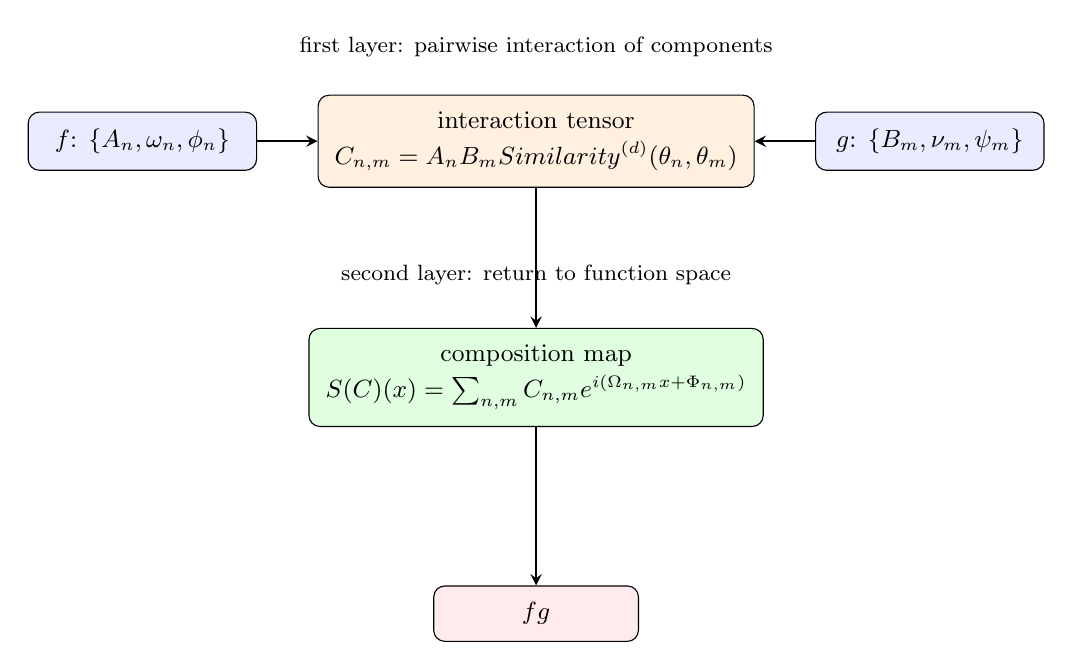
\begin{tikzpicture}[>=stealth,
  box/.style={draw, rounded corners, align=center, font=\small, inner sep=6pt}]
  \node[box, fill=blue!8, minimum width=2.9cm] (f) at (-5,1.5) {$f$: $\{A_n,\omega_n,\phi_n\}$};
  \node[box, fill=orange!12, minimum width=3.6cm] (C) at (0,1.5) {interaction tensor\\[2pt]$C_{n,m}=A_nB_m\operatorname{Similarity}^{(d)}(\theta_n,\theta_m)$};
  \node[box, fill=blue!8, minimum width=2.9cm] (g) at (5,1.5) {$g$: $\{B_m,\nu_m,\psi_m\}$};
  
  \node[box, fill=green!12, minimum width=3.9cm] (S) at (0,-1.5) {composition map\\[2pt]$S(C)(x)=\sum_{n,m}C_{n,m}e^{i(\Omega_{n,m}x+\Phi_{n,m})}$};
  
  \node[box, fill=red!8, minimum width=2.6cm] (out) at (0,-4.5) {$f\circledast g$};
  
  \draw[->,thick] (f) -- (C);
  \draw[->,thick] (g) -- (C);
  \draw[->,thick] (C) -- (S);
  \draw[->,thick] (S) -- (out);
  
  \node[font=\footnotesize] at (0,2.7) {first layer: pairwise interaction of components};
  \node[font=\footnotesize] at (0,-0.2) {second layer: return to function space};
\end{tikzpicture}
\caption{The two-layer construction of the convolution operator. The first layer pairs the components of the two epicycle families two by two, yielding a doubly indexed object (at $n\neq m$ this is a cross-frequency interaction); the second layer sends that object back to function space by means of the frequency composition operator $\Omega_{n,m}$ and the phase composition operator $\Phi_{n,m}$. The composite of the two layers is the convolution operator; when $\operatorname{Similarity}^{(d)}$ is taken to be a phase similarity kernel and $\Omega,\Phi$ take the sum-angle form, one obtains the periodic convolution $f\circledast g$.}
\label{fig:convolution_two_layers}
\end{figure}

\subsection{\texorpdfstring{Amplitude, Phase and Frequency Convolutions}{Amplitude, Phase and Frequency Convolutions}}

Let $f, g$ have period $T$ with frequency-series expansions
\[
f(t) = \sum_{m} c_m e^{i 2\pi m t/T}, \quad c_m = A_m e^{i\theta_m}; \qquad
g(t) = \sum_{n} d_n e^{i 2\pi n t/T}, \quad d_n = B_n e^{i\varphi_n}.
\]
where $A_m,B_n\ge 0$ are amplitudes, $\theta_m,\varphi_n\in[0,2\pi)$ are phases, and $\omega_m=2\pi m/T$, $\nu_n=2\pi n/T$ are frequencies.

\begin{definition}[Amplitude Convolution]\label{def:amplitude_convolution}
The \textbf{amplitude convolution} of $f$ and $g$ is the real matrix $\mathbb{A} = (\mathbb{A}_{mn})$:
\[
\mathbb{A}_{mn} := A_m B_n.
\]
The amplitude convolution discards all phase information and retains only the scale relations. $\mathbb{A}_{mn} \ge 0$ holds for all $m, n$.
\end{definition}

\begin{definition}[Phase Convolution]\label{def:phase_convolution}
The \textbf{phase convolution} of $f$ and $g$ is the complex matrix $\mathbb{P} = (\mathbb{P}_{mn})$:
\[
\mathbb{P}_{mn} := e^{i(\theta_m - \varphi_n)} = \cos(\theta_m - \varphi_n) + i\sin(\theta_m - \varphi_n).
\]
The phase convolution discards all amplitude information and retains only the directional relations. $|\mathbb{P}_{mn}| = 1$ holds for all $m, n$.
\end{definition}

\begin{definition}[Frequency Convolution]\label{def:frequency_convolution}
The \textbf{frequency convolution} of $f$ and $g$ is the real matrix $\mathbb{F} = (\mathbb{F}_{mn})$:
\[
\mathbb{F}_{mn} := \omega_m \nu_n = \frac{2\pi m}{T} \cdot \frac{2\pi n}{T} = \frac{4\pi^2 mn}{T^2}.
\]
The frequency convolution discards all amplitude and phase information and retains only the frequency-lattice structure. The frequency convolution is entirely determined by the fundamental period $T$.
\end{definition}

\begin{definition}[Trend Convolution]\label{def:tendency_convolution}
The \textbf{trend convolution} of $f$ and $g$ is the complex matrix $\mathbb{T} = (\mathbb{T}_{mn})$:
\[
\mathbb{T}_{mn} := A_m B_n \, \mathbb{P}_{mn} = A_m B_n e^{i(\theta_m - \varphi_n)} = c_m \overline{d_n}.
\]
Trend convolution $=$ amplitude convolution $\times$ phase convolution (term by term).
\end{definition}

\begin{proposition}[Relations among the Three Convolutions and Trend Convolution]\label{prop:three_convolutions_relation}
With the above notation:
\begin{enumerate}[label=(\roman*)]
    \item Trend convolution $=$ amplitude convolution $\times$ phase convolution: $\mathbb{T}_{mn} = \mathbb{A}_{mn} \mathbb{P}_{mn}$.
    \item Frequency convolution $=$ outer product of the frequency series: $\mathbb{F}_{mn} = \omega_m \nu_n$.
    \item In the frequency domain the three capture three independent components of convolution: amplitude (scaling), phase (rotation) and frequency (translation).
\end{enumerate}
\end{proposition}

\begin{proof}
(i) By Definitions \ref{def:amplitude_convolution} and \ref{def:phase_convolution}: $\mathbb{A}_{mn}\mathbb{P}_{mn} = A_m B_n e^{i(\theta_m - \varphi_n)} = \mathbb{T}_{mn}$.
(ii) By Definition \ref{def:frequency_convolution}.
(iii) From (i)(ii) and the definitions of the three.
\end{proof}

\begin{proposition}[Conjugate Symmetry of Phase Convolution]\label{prop:phase_convolution_symmetry}
The phase convolution matrix satisfies $\mathbb{P}_{mn} = \overline{\mathbb{P}'_{nm}}$, where $\mathbb{P}'_{mn} := e^{i(\varphi_m - \theta_n)}$ is the phase convolution obtained on interchanging the roles of $f$ and $g$. The amplitude and frequency convolutions are symmetric real matrices: $\mathbb{A}_{mn} = \mathbb{A}_{nm}$, $\mathbb{F}_{mn} = \mathbb{F}_{nm}$.
\end{proposition}

\begin{proof}
$\overline{\mathbb{P}_{nm}} = \overline{e^{i(\theta_n - \varphi_m)}} = e^{i(\varphi_m - \theta_n)}$, whilst $\mathbb{P}_{mn} = e^{i(\theta_m - \varphi_n)}$; in general the two are not equal. The correct symmetry is: defining $\mathbb{P}'_{mn} := e^{i(\varphi_m - \theta_n)}$, we have $\mathbb{P}'_{mn} = \overline{\mathbb{P}_{nm}}$. The symmetry of the amplitude and frequency convolutions follows directly from $A_m B_n = B_n A_m$ and $\omega_m \nu_n = \nu_n \omega_m$.
\end{proof}

\begin{remark}[Non-Symmetry of Phase Convolution]\label{rem:phase_convolution_asymmetry}
The phase convolution matrix is in general not symmetric: $\mathbb{P}_{mn} = e^{i(\theta_m - \varphi_n)}$ and $\mathbb{P}_{nm} = e^{i(\theta_n - \varphi_m)}$ are generally unequal, because the roles of $f$ and $g$ cannot be interchanged---$\theta_m$ comes from $f$ and $\varphi_n$ from $g$. Only after taking the complex conjugate is there the relation $\mathbb{P}_{mn} = \overline{\mathbb{P}'_{nm}}$, where $\mathbb{P}'_{mn} := e^{i(\varphi_m - \theta_n)}$ is the phase convolution obtained on interchanging the roles of $f$ and $g$. This contrasts with the symmetry of the amplitude and frequency convolutions.
\end{remark}

\begin{definition}[Kernelised Convolution (Master Kernel Decomposition Formula)]\label{def:kernelized_convolution}
Let the weight kernel be $W: \mathbb{R} \to \mathbb{C}$, the similarity kernels $S^{(d)}$ ($d = 1,\dots,6$) and the amplitude switch $\alpha \in \{0, 1\}$. Define the \textbf{kernelised convolution}
\[
\mathcal{K}^{(d)}_{W,\alpha}(\tau) := \sum_{m,n} W(\omega_m - \omega_n) \cdot (A_m B_n)^{\alpha} \cdot S^{(d)}(\theta_m, \varphi_n) \cdot e^{i\omega_n \tau}.
\]
\begin{enumerate}[label=(\roman*)]
    \item $\alpha = 0$: phase convolution (taking $S^{(d)}$ to be the $d$-dimensional phase kernel);
    \item $\alpha = 1$: trend convolution.
\end{enumerate}
\end{definition}

\begin{proposition}[The Six Complex Phase Kernels]\label{prop:six_complex_kernels}
The six complex phase kernels are generated from difference/sum angles and base/double/half angles:
\[
S^{(1)} = e^{i(\theta_m - \varphi_n)}, \quad S^{(2)} = e^{i(\theta_m + \varphi_n)}, \quad S^{(3)} = e^{i \cdot 2(\theta_m - \varphi_n)},
\]
\[
S^{(4)} = e^{i(\theta_m - \varphi_n)/2}, \quad S^{(5)} = e^{i \cdot 2(\theta_m + \varphi_n)}, \quad S^{(6)} = e^{i(\theta_m + \varphi_n)/2}.
\]
\end{proposition}

\begin{proof}
The 12 real similarity measures of the `Scalars and Vectors' chapter are precisely the real and imaginary parts of these 6 complex kernels (the cosine family and the sine family).
\end{proof}

\begin{lemma}[Windowed Expansion]\label{lem:windowed_expansion}
Let $w$ be an integrable window on $[-T, T]$ and let $\widehat{w}(\Omega) := \frac{1}{2T} \int_{-T}^{T} w(t) e^{i\Omega t}\,dt$. Then
\[
\frac{1}{2T}\int_{-T}^{T} f(t) e^{-i\Omega t} w(t)\,dt = \sum_{m} c_m\, \widehat{w}(\omega_m - \Omega).
\]
\end{lemma}

\begin{proof}
Substitute the frequency series of $f$ and integrate term by term using uniform convergence.
\end{proof}

\begin{theorem}[Window--Kernel Duality Theorem]\label{thm:window_kernel_duality}
Let $f, g$ have period $T$ and let $w$ be an even window. The windowed delay inner product
\[
(f \star_w g)(\tau) := \frac{1}{2T}\int_{-T}^{T} f(t)\, \overline{g(t - \tau)}\, w(t)\,dt
\]
has the expansion
\[
(f \star_w g)(\tau) = \sum_{m,n} \widehat{w}(\omega_m - \omega_n) \cdot c_m \overline{d_n} \cdot e^{i\omega_n \tau}.
\]
\end{theorem}

\begin{proof}
Substitute the frequency series and apply Lemma \ref{lem:windowed_expansion}.
\end{proof}

\begin{corollary}[Gaussian Window and Gaussian Kernel]\label{cor:gaussian_window_kernel}
Taking the Gaussian time window $w(t) = e^{-t^2/(2\sigma_t^2)}$, the frequency-domain kernel is a Gaussian kernel:
\[
\widehat{w}(\omega) \approx \frac{\sqrt{2\pi}\,\sigma_t}{2T}\, e^{-\sigma_t^2 \omega^2 / 2}.
\]
\end{corollary}

\begin{corollary}[Classical Limit: Rectangular Window and $\delta$ Kernel]\label{cor:classical_limit}
Taking the rectangular window $w(t) = \mathbf{1}_{[-T,T]}(t)$, we have $\widehat{w}(\omega) = \frac{\sin(\omega T)}{\omega T}$, and $\widehat{w}(\omega_m - \omega_n) \to \delta_{mn}$ as $T \to \infty$.
\end{corollary}

\begin{corollary}[Zero Delay and Cosine Similarity]\label{cor:zero_delay_cosine}
Taking $\tau = 0$ and normalising gives
\[
\frac{(f \star g)(0)}{\|f\| \|g\|}
\]
which is precisely the cosine similarity in $L^2([0,T])$.
\end{corollary}

\begin{property}[Basic Properties of Phase, Amplitude, Frequency, and Trend Convolutions]\label{prop:convolution_types_properties}
\begin{enumerate}[label=(\roman*)]
    \item $|\mathbb{P}_{mn}| = 1$, $\mathbb{P}_{mn} = \overline{\mathbb{P}'_{nm}}$, where $\mathbb{P}'_{mn} := e^{i(\varphi_m - \theta_n)}$ is the phase convolution obtained on interchanging the roles of $f$ and $g$ (subject to the convention on the domain of the phases, see Remark \ref{rem:phase_convolution_asymmetry});
    \item $\mathbb{A}_{mn} = \mathbb{A}_{nm} \ge 0$;
    \item $\mathbb{F}_{mn} = \mathbb{F}_{nm}$;
    \item $\mathbb{T}_{mn} = \mathbb{A}_{mn} \mathbb{P}_{mn} = \overline{\mathbb{T}_{nm}}$;
    \item time reversal interchanges the difference-angle family and the sum-angle family;
    \item the amplitude switch $\alpha$ going from $0$ to $1$ takes phase convolution to trend convolution.
\end{enumerate}
\end{property}

\begin{proof}
Each item is verified directly from the definitions.
\end{proof}

\begin{example}[Phase/Amplitude/Frequency Convolution Matrices for Period 2]\label{ex:period_two_matrix}
Let $T = 2$, $f(t) = c_0 + c_1 e^{i\pi t}$, $g(t) = d_0 + d_1 e^{i\pi t}$. Then:
\[
\mathbb{P} = \begin{pmatrix}
e^{i(\theta_0 - \varphi_0)} & e^{i(\theta_0 - \varphi_1)} \\
e^{i(\theta_1 - \varphi_0)} & e^{i(\theta_1 - \varphi_1)}
\end{pmatrix}, \quad
\mathbb{A} = \begin{pmatrix}
A_0 B_0 & A_0 B_1 \\
A_1 B_0 & A_1 B_1
\end{pmatrix}, \quad
\mathbb{T} = \begin{pmatrix}
c_0 \overline{d_0} & c_0 \overline{d_1} \\
c_1 \overline{d_0} & c_1 \overline{d_1}
\end{pmatrix}.
\]
The frequency convolution matrix is $\mathbb{F} = \begin{pmatrix} 0 & 0 \\ 0 & \pi^2 \end{pmatrix}$ ($\omega_0 = 0$, $\omega_1 = \pi$).
\end{example}

\begin{example}[Concrete Matrix for He Tu Phase Convolution]\label{ex:hetu_phase_convolution}
Take $T = 10$ and $f = g$ a He Tu complex function $f(z) = \sum_{n=0}^{9} c_n e^{2\pi i n z/10}$, where $c_n = A_n e^{i\phi_n}$. The phase convolution matrix $\mathbb{P}$ is a $10 \times 10$ matrix with entries $\mathbb{P}_{mn} = e^{i(\phi_m - \phi_n)}$. Under the decomposition $\mathbb{Z}_{10} \cong \mathbb{Z}_2 \times \mathbb{Z}_5$, $\mathbb{P}$ splits into four $5 \times 5$ blocks:
\[
\mathbb{P} = \begin{pmatrix} \mathbb{P}^{(\text{yang},\text{yang})} & \mathbb{P}^{(\text{yang},\text{yin})} \\ \mathbb{P}^{(\text{yin},\text{yang})} & \mathbb{P}^{(\text{yin},\text{yin})} \end{pmatrix},
\]
where the $(\text{yang},\text{yang})$ block corresponds to $m, n \in \{0,1,2,3,4\}$, the $(\text{yin},\text{yin})$ block to $m, n \in \{5,6,7,8,9\}$, and the cross blocks to the mixed yin--yang phase interaction.
\end{example}

\subsection{\texorpdfstring{Periodic Convolution: Complete Interaction of the Four-Parameter Operator}{Periodic Convolution}}
\label{subsec:periodic_convolution_series}

\begin{definition}[Periodic Convolution]\label{def:periodic_convolution}
Let $f, g$ be periodic functions (or almost periodic functions) with periodic-series expansions
\[
f(t) = \sum_{p \in P} \sum_{n \in \mathbb{Z}} A_{p,n} e^{i(\omega_{p,n} t + \phi_{p,n})}, \qquad
g(t) = \sum_{q \in Q} \sum_{m \in \mathbb{Z}} B_{q,m} e^{i(\nu_{q,m} t + \psi_{q,m})},
\]
where $\omega_{p,n} = 2\pi n / T_p$ and $\nu_{q,m} = 2\pi m / T_q$. Define the \textbf{frequency composition operator} and the \textbf{phase composition operator} by
\[
\Omega_{p,q,n,m} := \omega_{p,n} + \nu_{q,m}, \qquad
\Phi_{p,q,n,m} := \phi_{p,n} + \psi_{q,m} \pmod{2\pi}.
\]
The \textbf{periodic convolution} of $f$ and $g$ is defined as
\[
(f \circledast g)(t) = \sum_{p \in P} \sum_{q \in Q} \sum_{n, m \in \mathbb{Z}} A_{p,n} B_{q,m} \cdot \operatorname{Similarity}^{(d)}(\theta_{p,n}, \theta_{q,m}) \cdot e^{i(\Omega_{p,q,n,m} t + \Phi_{p,q,n,m})},
\]
where:
\begin{itemize}
    \item $\theta_{p,n} = (\omega_{p,n}, \phi_{p,n})$ is the phase point of the $(p,n)$-th component of $f$;
    \item $\theta_{q,m} = (\nu_{q,m}, \psi_{q,m})$ is the phase point of the $(q,m)$-th component of $g$;
    \item $\operatorname{Similarity}^{(d)}$ is the $d$-dimensional phase similarity kernel ($d = 1, \dots, 6$, corresponding to the 6 complex phase kernels, Proposition \ref{prop:six_complex_kernels}).
\end{itemize}
Periodic convolution takes the four parameters \textbf{amplitude} (scaling), \textbf{frequency} (translation), \textbf{phase} (rotation) and \textbf{period} (fixed length) as its operators, preserving the interaction of all frequency pairs and all period pairs. When $P = Q = \{T\}$ (a single period layer) and only the diagonal terms $n = m$ are retained, periodic convolution degenerates to classical convolution (Definition \ref{def:convolution}).
\end{definition}

\begin{proposition}[Degenerate Cases of Periodic Convolution]\label{prop:periodic_convolution_degenerations}
\begin{enumerate}[label=(\roman*)]
    \item \textbf{Single period layer + diagonal kernel}: $P = Q = \{T\}$, $W \to \delta_{nm}$, $S^{(1)}$ (difference angle), $\alpha = 1$; then periodic convolution degenerates to classical convolution:
    \[
    (f \circledast g)(t) \to (f * g)(t) = \sum_n c_n d_n e^{i\omega_n t}.
    \]
    \item \textbf{Single period layer + full matrix}: $P = Q = \{T\}$, $W \equiv 1$, $S^{(1)}$, $\alpha = 1$; then periodic convolution degenerates to trend convolution:
    \[
    (f \circledast g)_{n,m} = \mathbb{T}_{nm} = c_n \overline{d_m}.
    \]
    \item \textbf{Single period layer + unit modulus}: $P = Q = \{T\}$, $W \equiv 1$, $S^{(1)}$, $\alpha = 0$; then periodic convolution degenerates to phase convolution:
    \[
    (f \circledast g)_{n,m} = \mathbb{P}_{nm} = e^{i(\theta_n - \varphi_m)}.
    \]
\end{enumerate}
\end{proposition}

\begin{proof}
(i) When $W \to \delta_{nm}$ the off-diagonal terms disappear and only the terms $n = m$ remain. From $S^{(1)}(n,n) = 1$ and $\Phi_{n,n} = \theta_n + \varphi_n$ we obtain $\sum_n A_n B_n e^{i(2\omega_n t + \theta_n + \varphi_n)} = \sum_n c_n d_n e^{i\omega_n t}$.
(ii) When $W \equiv 1$ all frequency pairs are retained, and $\alpha = 1$ retains the amplitude products, giving the trend convolution matrix $\mathbb{T}_{nm} = c_n \overline{d_m}$.
(iii) With $W \equiv 1$, $\alpha = 0$ discards the amplitudes, giving the phase convolution matrix $\mathbb{P}_{nm} = e^{i(\theta_n - \varphi_m)}$.
\end{proof}

\begin{theorem}[Functoriality of Periodic Convolution]\label{thm:periodic_convolution_functoriality_series}
Periodic convolution $\circledast$ is a bifunctor on the translation-periodic category, satisfying:
\begin{enumerate}[label=(\roman*)]
    \item \textbf{Preservation of identities}: $\operatorname{id}_f \circledast \operatorname{id}_g = \operatorname{id}_{f \circledast g}$.
    \item \textbf{Preservation of composition}: $(h_2 \circ h_1) \circledast (k_2 \circ k_1) = (h_2 \circledast k_2) \circ (h_1 \circledast k_1)$.
    \item \textbf{Compatibility with phase convolution}: $\mathbb{P}(f \circledast g) \cong \mathbb{P}(f) \otimes \mathbb{P}(g)$.
    \item \textbf{Compatibility with trend convolution}: $\mathbb{T}(f \circledast g) \cong \mathbb{T}(f) \otimes \mathbb{T}(g)$.
\end{enumerate}
\end{theorem}

\begin{proof}
(i)--(ii) Are guaranteed by the linearity of periodic convolution and the functoriality of the Fourier transform. (iii)--(iv) Are verified directly from the frequency-domain representation of periodic convolution (the outer product $\mathbf{c}_f \otimes \mathbf{c}_g$) and the definitions of phase and trend convolution. Periodic convolution is a tensor product in the frequency domain, whilst phase and trend are pointwise operations in the frequency domain.
\end{proof}

\begin{proposition}[Relation between Periodic Convolution and the Four Classical Convolutions]\label{prop:periodic_convolution_hierarchy}
Periodic convolution is the summit of the five-stage ladder of convolution theory, and the degeneration relations between the successive stages are:
\[
\text{periodic convolution} \circledast \xrightarrow{\text{single period layer}} \text{trend convolution} \mathbb{T} \xrightarrow{\text{diagonal kernel } W \to \delta} \text{classical convolution} *,
\]
\[
\text{periodic convolution} \circledast \xrightarrow{\text{single period layer} + \alpha = 0} \text{phase convolution} \mathbb{P}.
\]
In addition, trend convolution $=$ amplitude convolution $\times$ phase convolution (term by term), and frequency convolution $=$ the outer product of the frequency series; the three describe convolution from the three independent components of amplitude, phase and frequency.
\end{proposition}

\begin{proof}
It follows directly from Proposition \ref{prop:periodic_convolution_degenerations} and \ref{prop:three_convolutions_relation}.
\end{proof}

\begin{remark}[The Complete Hierarchy of Five Stages]\label{rem:five_stage_hierarchy}
The five-stage ladder of convolution theory is: \textbf{classical convolution} (retaining only the delay products of equal frequency pairs $m = n$) $\to$ \textbf{phase convolution/amplitude convolution/frequency convolution} (retaining the phase, amplitude and frequency components of all frequency pairs respectively) $\to$ \textbf{trend convolution} (retaining the amplitudes and phases of all frequency pairs) $\to$ \textbf{periodic series} (decomposition into multiple period layers) $\to$ \textbf{periodic convolution} (a four-parameter operator, retaining the interaction of all frequency pairs and all period pairs). Each stage of the five-stage ladder is a degeneration of the preceding one, and the information content strictly increases from stage to stage.
\end{remark}

\begin{figure}[htbp]
\centering
\begin{tikzpicture}[scale=0.9,>=stealth,
  node distance=1.1cm,
  ladder/.style={draw, rounded corners, minimum width=11.0cm, minimum height=0.8cm, align=center, font=\small},
  arrow/.style={->, thick, >=stealth}]

  \node[ladder, fill=blue!10] (s1) {classical convolution $f * g = \sum_n c_n d_n e^{i\omega_n t}$ (equal frequency pairs only)};
  \node[ladder, fill=cyan!12, below=of s1] (s2) {phase convolution / amplitude convolution / frequency convolution (single-component projections of all frequency pairs)};
  \node[ladder, fill=green!12, below=of s2] (s3) {trend convolution $\mathbb{T}_{mn} = c_m \overline{d_n}$ (amplitudes and phases of all frequency pairs)};
  \node[ladder, fill=orange!12, below=of s3] (s4) {periodic series (decomposition into multiple period layers, parametrised by four-tuples)};
  \node[ladder, fill=red!15, below=of s4] (s5) {periodic convolution $f \circledast g$ (a four-parameter operator, all frequency pairs and all period pairs)};

  \draw[arrow] (s1) -- node[right, font=\scriptsize, text=gray!70!black, align=left] {degeneration} (s2);
  \draw[arrow] (s2) -- node[right, font=\scriptsize, text=gray!70!black, align=left] {synthesis} (s3);
  \draw[arrow] (s3) -- node[right, font=\scriptsize, text=gray!70!black, align=left] {layering} (s4);
  \draw[arrow] (s4) -- node[right, font=\scriptsize, text=gray!70!black, align=left] {four-parameterisation} (s5);

  \node[font=\scriptsize, gray!70!black, align=center] at (7.5,-3.6) {information content strictly increasing};
\end{tikzpicture}
\caption{The five-stage ladder of convolution theory. From classical convolution (the simplest, equal frequency pairs only) to periodic convolution (the summit, four-parameterised), each stage is a degeneration or a synthesis of the preceding one, and the information content strictly increases. Periodic convolution simultaneously retains the complete interaction information of the four components amplitude, frequency, phase and period.}
\label{fig:convolution_five_stages}
\end{figure}

\begin{property}[The core parametrisation of the periodic convolution]\label{prop:periodic_convolution_parametrization}
Periodic convolution (Definition \ref{def:periodic_convolution}) takes four parameters as its operators:
\begin{enumerate}[label=(\roman*)]
  \item \textbf{Amplitude} (scaling): the amplitude switch $\alpha$ controls whether the amplitude products $A_{p,n} B_{q,m}$ are retained;
  \item \textbf{Frequency} (translation): the frequency composition operator $\Omega_{p,q,n,m} = \omega_{p,n} + \nu_{q,m}$ composes new frequencies;
  \item \textbf{Phase} (rotation): the phase similarity kernel $\operatorname{Similarity}^{(d)}(\theta_{p,n}, \theta_{q,m})$ retains the phase relations;
  \item \textbf{Period} (fixed length): the set of period-class indices $P \times Q$ retains the interaction of all period pairs.
\end{enumerate}
The complete retention of the four parameters makes periodic convolution the operator with the greatest information content in convolution theory.
\end{property}

\begin{proof}
From the explicit formula for periodic convolution in Definition \ref{def:periodic_convolution}, the four parameters appear in four factors respectively: the amplitude $A_{p,n}B_{q,m}$, the frequency composition $\Omega_{p,q,n,m}$, the phase kernel $\operatorname{Similarity}^{(d)}$ and the period index $P \times Q$. Proposition \ref{prop:periodic_convolution_degenerations} shows that removing any one parameter degenerates the operator to the next stage of the ladder.
\end{proof}

\section*{Seven-theme comparison table for this chapter}

\begin{center}
\renewcommand{\arraystretch}{1.3}
\begin{tabular}{>{\centering\arraybackslash}p{2.2cm}>{\centering\arraybackslash}p{10.5cm}}
\toprule
Theme & Corresponding content in this chapter \\
\midrule
Translation & the local translation expansion of the Taylor series; the global translation period of the Fourier series; the translation property of convolution (Proposition \ref{prop:convolution_properties}); the half-period translation of He Tu complex functions (Proposition \ref{prop:hetu_yin_yang_flip}) \\
Scaling & the amplitude series (Definition \ref{def:amplitude_series}); amplitude convolution (Definition \ref{def:amplitude_convolution}); the amplitude products of trend convolution (Definition \ref{def:tendency_convolution}) \\
Rotation & the phase series (Definition \ref{def:phase_series}); phase convolution (Definition \ref{def:phase_convolution}); the 6 complex phase kernels (Proposition \ref{prop:six_complex_kernels}); the He Tu phase operator (Definition \ref{def:hetu_phase_operator}) \\
Conservation & Parseval's identity (Theorem \ref{thm:parseval_fourier_classical}); Parseval's identity for the amplitude series (Proposition \ref{prop:amplitude_parseval}); Bohr's generalised Parseval identity (Theorem \ref{thm:bohr_parseval}) \\
Symmetry & the positive--negative power symmetry of the Laurent series; the orthogonal symmetry of the Fourier basis (Proposition \ref{prop:fourier_orthogonality}); the symmetry of amplitude and frequency convolutions (Proposition \ref{prop:convolution_types_properties}); the direct product decomposition of the He Tu phase operator group (Proposition \ref{prop:hetu_phase_group}) \\
Closure & the uniqueness of the coefficients of the periodic series (Theorem \ref{thm:periodic_series_bohr}); the functorial closure lattice of periodic convolution (Theorem \ref{thm:periodic_convolution_functoriality_series}) \\
Period & the frequency series (Definition \ref{def:frequency_series}); the four-tuple structure of the periodic series (Definition \ref{def:periodic_series}); the five-stage ladder of periodic convolution (Proposition \ref{prop:periodic_convolution_hierarchy}); the period structure of the He Tu five-phase components (Proposition \ref{prop:hetu_five_periods}) \\
\bottomrule
\end{tabular}
\end{center}

\section*{Exercises}

\begin{enumerate}[leftmargin=3em, label=\textbf{Exercise \arabic*}]
    \item Prove the ratio test and the root test (Proposition \ref{prop:ratio_root_tests}):
    let $a_k\neq0$; if
    \[
    \lim_{k\to\infty}\left|\frac{a_{k+1}}{a_k}\right|=\rho
    \quad\text{or}\quad
    \lim_{k\to\infty}\sqrt[k]{|a_k|}=\rho,
    \]
    then the series converges absolutely when $\rho<1$, diverges when $\rho>1$, and the test is inconclusive when $\rho=1$.
    Please write out complete proofs of the two tests separately, and give one example of failure when $\rho=1$ for each of them.

    \item Prove the Weierstrass $M$-test (Theorem \ref{thm:weierstrass_mtest}):
    let $\sum_k M_k$ converge and let $|u_k(t)|\le M_k$ for all $t\in I$;
    then $\sum_k u_k(t)$ converges uniformly and absolutely on $I$.
    Then prove term-by-term integration under uniform convergence (Theorem \ref{thm:uniform_termwise_integration}) and term-by-term differentiation
    (Theorem \ref{thm:uniform_termwise_differentiation}).

    \item Find the convergence condition and the sum function of the geometric series $\sum_{k=0}^{\infty}r^k$ (Example \ref{ex:geometric_series}),
    and use it to derive:
    \begin{enumerate}[label=(\roman*)]
        \item $\displaystyle \sum_{k=0}^{\infty}kr^k=\frac{r}{(1-r)^2}$ ($|r|<1$);
        \item $\displaystyle \sum_{k=0}^{\infty}k^2r^k=\frac{r(1+r)}{(1-r)^3}$ ($|r|<1$).
    \end{enumerate}

    \item Write out the Taylor series of $e^x$, $\sin x$, $\cos x$, $\ln(1+x)$ and $(1+x)^\alpha$
    (Example \ref{ex:taylor_examples}), and use the Taylor formula with Lagrange remainder
    (Theorem \ref{thm:taylor_lagrange}) to prove that
    \[
    e^x=\sum_{k=0}^{\infty}\frac{x^k}{k!}
    \]
    holds for all $x\in\mathbb{R}$.
    Further explain the local--global duality between the Taylor expansion and the Fourier expansion (Remark \ref{rem:taylor_fourier_duality}).

    \item Verify the uniqueness of the coefficients of a Laurent series (Lemma \ref{lem:laurent_uniqueness}),
    and write out the Laurent expansion of $e^{1/z}$ on $|z|>0$ (Example \ref{ex:laurent_example}).
    According to the form of the principal part, determine which type of singularity $z_0=0$ is for $e^{1/z}$
    (Proposition \ref{prop:laurent_singularity}).

    \item Let $f$ have period $T$ and be integrable on $[0,T]$, with complex Fourier coefficients $c_n$.
    Prove the orthogonality of the Fourier basis (Proposition \ref{prop:fourier_orthogonality}):
    \[
    \frac{1}{T}\int_0^T e^{i2\pi(n-m)t/T}\,dt=\delta_{nm}.
    \]
    And use orthogonality to prove Parseval's identity (Theorem \ref{thm:parseval_fourier_classical}):
    \[
    \frac{1}{T}\int_0^T|f(t)|^2\,dt=\sum_{n\in\mathbb{Z}}|c_n|^2.
    \]

    \item Write out the Fourier series of the square wave (taking $1$ on $[0,T/2)$ and $-1$ on $[T/2,T)$)
    (Example \ref{ex:fourier_square_wave}).
    Explain the convergence value given by the Dirichlet convergence theorem (Theorem \ref{thm:dirichlet_convergence}) at the jump point,
    and explain why the Gibbs phenomenon (Example \ref{ex:gibbs_phenomenon}) does not disappear as the number of terms increases.

    \item Prove the Fej\'er kernel and uniform convergence theorem (Theorem \ref{thm:fejer_uniform}):
    let $f$ be continuous and have period $T$; the Fej\'er means
    \[
    \sigma_Nf(t)=\frac{1}{N+1}\sum_{k=0}^{N}S_kf(t)
    \]
    converge uniformly to $f$ on $\mathbb{R}$.
    Please explain that the Fej\'er kernel is a good kernel (non-negative, of integral $1$, tending to zero uniformly away from the origin),
    and explain why the Fej\'er means can avoid the Gibbs phenomenon.

    \item Prove the He Tu Fourier decomposition (Theorem \ref{thm:hetu_fourier_decomposition}):
    let $f$ satisfy $f(z+10)=f(z)$ and let its Fourier expansion converge uniformly; then
    \[
    f(z)=\sum_{k=0}^{4}\left(c_k+c_{k+5}e^{\pi iz}\right)e^{2\pi ikz/10}.
    \]
    Taking the concrete function
    \[
    f(z)=3+2e^{\pi iz/5}+e^{\pi iz}+5e^{3\pi iz/5}+4e^{2\pi iz},
    \]
    write out its five $\mathbb{Z}_5$ components, and verify that the half-period translation $z\mapsto z+5$ changes the sign of the odd components
    (Proposition \ref{prop:hetu_yin_yang_flip}).

    \item Prove the relation between the phase series and time translation (Proposition \ref{prop:phase_translation}):
    if $\mathcal{P}_f(t)=\sum_n e^{i(nt+\phi_n)}$,
    then the time translation $f_\tau(t)=f(t-\tau)$ corresponds to rotating each term of the phase series by $-n\tau$.
    Then prove modulus conservation for finite phase series (Theorem \ref{thm:phase_modulus_conservation}):
    \[
    \frac{1}{2\pi}\int_0^{2\pi}|S_N(t)|^2dt=2N+1.
    \]

    \item Prove Parseval's identity for the amplitude series (Proposition \ref{prop:amplitude_parseval}):
    let $f\in L^2([0,2\pi])$ have Fourier coefficients $c_n=A_ne^{i\phi_n}$; then
    \[
    \frac{1}{2\pi}\int_0^{2\pi}|f(t)|^2dt=\sum_{n\in\mathbb{Z}}A_n^2.
    \]
    And explain that the energy is determined by the amplitude spectrum alone and is independent of the phase spectrum (Corollary \ref{cor:amplitude_energy_only}).

    \item Prove the degenerate cases of periodic convolution (Proposition \ref{prop:periodic_convolution_degenerations}):
    \begin{enumerate}[label=(\roman*)]
        \item for a single period layer with $W\to\delta_{nm}$, $S^{(1)}$ and $\alpha=1$,
              periodic convolution degenerates to classical convolution;
        \item for a single period layer with $W\equiv1$, $S^{(1)}$ and $\alpha=1$,
              periodic convolution degenerates to trend convolution $\mathbb{T}_{nm}=c_n\overline{d_m}$;
        \item for a single period layer with $W\equiv1$, $S^{(1)}$ and $\alpha=0$,
              periodic convolution degenerates to phase convolution $\mathbb{P}_{nm}=e^{i(\theta_n-\varphi_m)}$.
    \end{enumerate}

    \item Synthesis problem: explain that the amplitude series, the phase series and the frequency series are respectively the projections of the periodic series onto its three components
    (Proposition \ref{prop:periodic_series_synthesis} and Corollary \ref{cor:periodic_series_projections}).
    Taking the periodic series
    \[
    f(t)=3e^{i(\sqrt{2}t+\pi/6)}+2e^{i(t-\pi/3)}
    \]
    as an example, write out explicitly its amplitude series, phase series and frequency series respectively,
    and point out why any single projection is insufficient to reconstruct $f$.
\end{enumerate}

